%\documentclass[german,a4paper,12p,headsepline, titlepage, liststotoc, idextotoc,bibtoctoc,blibliography = totocnumbered,left=40mm,right=20mm,top=25mm,bottom=20mm]{scrartcl}
\documentclass[german,a4paper, 12pt]{llncs}
\usepackage[left=30mm,right=30mm,top=25mm,bottom=25mm]{geometry}
\setlength{\footskip}{6mm} % Abstand Seitenzahl zu Text
\setcounter{tocdepth}{2}
\makeatletter
\renewcommand*\l@author[2]{}
\renewcommand*\l@author[2]{}
\makeatletter
\usepackage[utf8]{inputenc}
\usepackage[backend=biber,sorting =none]{biblatex}
\usepackage{csquotes}
\usepackage{graphicx}
\usepackage{babel}
\usepackage{subcaption}
\usepackage{mwe}
\usepackage[toc, page]{appendix}

\usepackage{parskip}
\usepackage{float}
%\usepackage{hbrs-inf}

%\usepackage{hyperref}
\usepackage{filecontents}
\usepackage{xcolor}
\usepackage{listings}

\lstdefinestyle{DOS}
{
	backgroundcolor=\color{black},
	basicstyle=\fontsize{11}{11}\color{white}\ttfamily
}


\begin{filecontents}{references.bib}
	

@article{averageHairshedding,
	author = {Sinclair, Rodney},
	year = {2015},
	month = {04},
	pages = {},
	title = {Hair Shedding In Women: How much is too much?},
	volume = {173},
	journal = {The British journal of dermatology},
	doi = {10.1111/bjd.13873}
}

@article{visualScale,
	author = {Martínez-Velasco, María and Vázquez-Herrera, Norma and Maddy, Austin and Asz-Sigall, Daniel and Tosti, Antonella},
	year = {2017},
	month = {02},
	pages = {},
	title = {The Hair Shedding Visual Scale: A Quick Tool to Assess Hair Loss in Women},
	volume = {7},
	journal = {Dermatology and Therapy},
	doi = {10.1007/s13555-017-0171-8}
}

@article{seasoalShedding,
	
	author = {Hsiang, E.Y. and Semenov, Yevgeniy and Aguh, Crystal and Kwatra, S.G.},
	year = {2017},
	month = {10},
	pages = {},
	title = {Seasonality of hair loss: a time series analysis of Google Trends data 2004 to 2016},
	volume = {178},
	journal = {British Journal of Dermatology},
	doi = {10.1111/bjd.16075}
}

@inbook{chemicalAlopecia,
	author = {Maibach, Howard and Yamaguchi, Ian},
	year = {2012},
	month = {01},
	pages = {1935-1942},
	title = {Chemically Induced Hair Loss/Alopecia},
	isbn = {978-3-642-02034-6},
	journal = {Kanerva's Occupational Dermatology, Second Edition},
	doi = {10.1007/978-3-642-02035-3_205}
}

@article{ironDeficiency,
	author = {Trost, Leonid and Bergfeld, Wilma and Calogeras, Ellen},
	year = {2006},
	month = {06},
	pages = {824-44},
	title = {The diagnosis and treatment of iron deficiency and its potential relationship to hair loss},
	volume = {54},
	journal = {Journal of the American Academy of Dermatology},
	doi = {10.1016/j.jaad.2005.11.1104}
}

@ONLINE{Canny,
	title = {Canny Edge Detector},
	url = {https://docs.opencv.org/master/da/d5c/tutorial_canny_detector.html},
	urldate = {2020-04-17},
}

@article{Watershed,
	author = {Kornilov, Anton and Safonov, Ilia},
	year = {2018},
	month = {10},
	pages = {123},
	title = {An Overview of Watershed Algorithm Implementations in Open Source Libraries},
	volume = {4},
	journal = {Journal of Imaging},
	doi = {10.3390/jimaging4100123}
}

@ONLINE{WatershedCV,
	title = {Image Segmentation with Watershed Algorithm},
	url = {https://opencv-python-tutroals.readthedocs.io/en/latest/py_tutorials/py_imgproc/py_watershed/py_watershed.html},
	urldate = {2020-04-17}
}

@ONLINE{TemplateMatchingCV,
	title = {Template Matching},
	url = {https://docs.opencv.org/2.4/doc/tutorials/imgproc/histograms/template_matching/template_matching.html},
	urldate = {2020-04-17}
}

@ONLINE{Matplotlib,
	title = {Matplotlib},
	url = {https://matplotlib.org/},
	urldate = {2020-04-17}
}

@ONLINE{Numpy,
	title = {Numpy},
	url = {https://numpy.org/},
	urldate = {2020-04-17}
}

@ONLINE{DilationCV,
	title = {Eroding and Dilating},
	url = {https://docs.opencv.org/2.4/doc/tutorials/imgproc/erosion_dilatation/erosion_dilatation.html},
	urldate = {2020-04-17}
}

@ONLINE{ConnectedComponents,
	title = {Connected Components in OpenCV},
	url = {https://davidlavy.wordpress.com/opencv/connected-components-in-opencv/},
	urldate = {2020-04-17}
}

@ONLINE{skel,
	title = {Skeletonize},
	url = {https://scikit-image.org/docs/dev/auto_examples/edges/plot_skeleton.html},
	urldate = {2020-04-17}
}

@inproceedings{outlierRemoval,
	author = {Amidan, B.G. and Ferryman, Thomas and Cooley, Scott},
	year = {2005},
	month = {04},
	pages = {3814 - 3819},
	title = {Data outlier detection using the Chebyshev theorem},
	journal = {Proc. IEEE Aerosp. Conf.},
	doi = {10.1109/AERO.2005.1559688}
}

@ONLINE{curveFittingIntro,
	title = {Introduciton to Curve Fitting},
	url = {https://www.ncss.com/wp-content/themes/ncss/pdf/Procedures/NCSS/Introduction_to_Curve_Fitting.pdf},
	urldate = {2020-04-17}
}
@ONLINE{curveFittingScipy,
	title = {scipy curve fit},
	url = {https://docs.scipy.org/doc/scipy/reference/generated/scipy.optimize.curve_fit.html},
	urldate = {2020-04-17}
}
@ONLINE{splineScipy,
	title = {scipy InterpolatedUnivariateSpline},
	url = {https://docs.scipy.org/doc/scipy/reference/generated/scipy.interpolate.InterpolatedUnivariateSpline.html},
	urldate = {2020-04-17}
}
@ONLINE{opencv,
	title = {Open CV},
	url = {https://opencv.org/},
	urldate = {2020-04-17}
}



\end{filecontents}

\addbibresource{references.bib}
\title{Praxisprojekt}
\subtitle{Automatisches Schätzen der Haaranzahl in ausgefallenen Haarbüscheln}
\author{\parbox{.9\textwidth}{\centering 
		\large Janelle Pfeifer \\
		\small Delpstraße 28\\
		53359 Rheinbach \\
		janelle.pfeifer@smail.inf.h-brs.de}}
\institute{\parbox{.9\textwidth}{\centering 
		\large Hochschule Bonn-Rhein-Sieg \\
		\normalsize Institute of Visual Computing \\ 
		\small Fachbereich Informatik \\
		Studiengang: Informatik (B.SC.)\\
		\normalsize Rheinbach, 24.4.2020}}
\date{Rheinbach, 24.4.2020}

\begin{document}
	%{\let\newpage\relax\maketitle}
	\maketitle
	\newpage
	\begin{abstract}
		Vermehrter Haarverlust kann ein Anzeichen von Krankheiten oder Mangelerscheinungen sein.
		
		In dieser Arbeit wird ein Verfahren vorgestellt, mit dem die Anzahl an ausgefallenen Haaren auf einem Bild, mithilfe von Methoden der Bildverarbeitung und statistischer Auswertung, geschätzt werden kann.
		
		So kann der tägliche Haarausfall effizient und effektiv überwacht werden.

	\end{abstract}
	\newpage
	\tableofcontents
	\newpage

\section{Einleitung}
%Die Einleitung ist mit der wichtigste Teil der Arbeit, da sie den Leser motivieren soll die vorliegende Arbeit weiter z lesen. Sie sollte neben einer Motivation bzw Problembeschreibung auch das Ziel der Arbeit beschreiben.Zusätzlich sollten die Fabgebiete die die arbeit betreffen und deren Bedeutung genannt werden. Wichtig ist eine klare Formulierung der Zielstellung und des Lösungsansatzes so wie abschließend eine Beschreibung der Gliederung der Arbeit.

Das Ausfallen von Haarsträhnen ist ein natürlicher Teil des Haarwachstum-Zyklus. Durchschnittlich verliert der Mensch 50 bis 150 Haarsträhnen am Tag. Vermehrter Haarausfall kann ein Anzeichen von Krankheiten oder Mangelerscheinungen sein.\cite{averageHairshedding}

Haarausfall ist sehr variabel und wird durch viele Faktoren beeinflusst. Er kann sich abhängig von dem Haartyp, der Haarlänge und der Haarpflege-Methode jeden Tag ändern und Muster aufweisen. Jeder Mensch hat ein eigenes Haarausfall-Muster. Eine Langzeitüberwachung gibt die Möglichkeit diese Muster zu erkennen und Abweichungen herauszustellen. \cite{chemicalAlopecia,ironDeficiency,seasoalShedding}

In dem Paper \blockquote{The Hair shedding visual scale: A quick tool to assess hair loss in Women} wird eine Methode beschrieben, in der Frauen anhand von Bildern den Umfang ihres täglichen Haarausfalls bestimmen können. Dabei wird den Frauen Bilder von abgezählten, ausgefallenen Haarbüscheln gezeigt, die ihrer eigenen Haarlänge entsprechen. Die Frauen wählen das Foto aus, welches ihrem persönlichen täglichen Haarausfall entspricht. Dabei wurde eine Korrelation festgestellt zwischen Frauen, die klinisch bestätigt Haarverlust erfahren und den Bildern, die sie auswählen.
Der Haarausfall kann somit visuell, anhand von Bildern festgestellt werden.\cite{visualScale}

In dieser Arbeit wird ein Verfahren vorgestellt, mit dem die Haaranzahl auf einem Bild von Methoden der Bildverarbeitung und statistischer Auswertung geschätzt werden kann. So wird eine Langzeitüberwachung möglichst effizient durchführbar.
\section{Grundlagen}
\subsection{Computervision}
In dem Bereich der Bildverarbeitung gibt es viele Algorithmen, die es ermöglichen Objekte in einem Bild erkennbar zu machen und zu verarbeiten.

\subsection{Template Matching} 

Template Matching findet Bereiche eines Bildes, die einem gegebenen Bild (Template) ähnlich sind.\cite{TemplateMatchingCV}

Dazu wird ein Source Image und ein Template Image angegeben. Um die gesuchten Bereiche zu finden, wird das Template Image Pixelweise über das Source Image geschoben. An jeder Stelle wird das Template mit dem Source Image verglichen und die Ähnlichkeit zwischen den Beiden berechnet. Als Ergebnis erhält man eine Matrix die für jeden Pixel des Bildes eine Wahrscheinlichkeit dafür angibt, das sich dort das Template befindet.\cite{TemplateMatchingCV}

\subsection{Canny Edge Detection}
Canny Edge Detection ist ein Algorithmus der Kanten in einem Bild erkennt. 
Es handelt sich um einen Hochpassfilter. Diese suchen nach Stellen im Bild, wo sich die Farben bzw. Graustufen stark voneinander unterscheiden. Solche Stellen heißen Hochfrequent. Linien und Kanten weisen eine Hohe Frequenz auf. Niederfrequente Bereiche weisen eine einheitlichere Farbe oder Graustufe auf. Ein Hochpassfilter lässt hochfrequente Bildanteile stehen und schwächt Niederfrequente ab. \cite{Canny}

Die Canny Edge Detection wird auf Graustufenbilder angewandt. An jeder Stelle des Bildes wird ein 3x3 Ausschnitt der Nachbarpixel betrachtet. Weisen die Nachbarpixel ein bestimmtest Muster auf, indem sie eine Linie beschreiben mit helleren Pixel auf einer Seite und dunkleren Pixeln auf der Anderen, wird die Stelle als Teil einer Kante betrachtet.\cite{Canny}


\subsection{Dilatation}
Die Dilatation arbeitet auf binären Bildern. Es gibt nur schwarz und weiß.
Die Dilatation fügt weiße Pixel an die Ränder von weißen Objekten hinzu. 
Es handelt es sich um ein Morpholigschen Operator und arbeitet somit das Bild Pixelweise durch. Der Wert jedes Pixels basiert auf einem Vergleich zwischen dem Pixel und dessen Nachbar-Pixeln.\cite{DilationCV}
	
\subsection{Inversion eines Graustufenbildes}

Die Graustufenwerte eines Bildes werden invertiert. 
Schwarz wird Weiß und Weiß wird Schwarz, helle Graustufen werden dunkel und umgekehrt.
 
Die Graustufen eines Bildes werden in 8 bit dargestellt. Somit gibt es 255 Graustufen. 0 ist schwarz und 255 ist weiß. 
Somit gilt bei der Inversion für jedes Pixel mit dem Graustufenwert g:

$g_{neu} = 255- g_{alt} $

\subsection{Watershed Algorithmus}

Der Watershed Algorithmus ist ein Region Growth Algorithmus. Er finden zusammenhängende Gruppen an Pixeln, die einander ähnlich sind. Diese Gruppen werden als Regionen bezeichnen. 

Für den Watershed Algorithmus wird zunächst in jede Region, die der Algorithmus wachsen lassen soll, eine Markierung, ein seed, gesetzt. Für die seeds werden die Pixel, die dem seed ähnlich sind zu der Region zusammengefasst. So wachsen die Regionen, bis sie auf eine andere Region stoßen.\cite{Watershed,WatershedCV}

Das Prinzip liegt darin die Graustufenwerte des Bildes als eine Topologische Karte anzusehen. Jeder seed liegt in einem Tal, in das Wasser hineingefühlt wird. Die Grenzen zwischen den Regionen liegen dort, wo das Wasser aus unterschiedlichen Tälern aufeinander trifft.\cite{Watershed,WatershedCV} 

\subsection{Connected Components}

Connected Components sind benachbarte Pixel, die denselben Grauwert haben. \cite{ConnectedComponents}

\subsection{Skelettierung}
Bei der Skelettierung werden Objekte binären Bildes auf nur eine Pixelbreite reduziert. Dabei Gelten Objekte als Connected Components. So können Linien auf eine Pixelbreite geschrumpft werden.\cite{skel}

\subsection{Outlier Removal}

Outlier Removal ist ein Prozess, der statistische Ausreißer entfernt. 
Basierend auf dem Tschebyscheff Theorem, wird der Mittelwert und die Varianz eines Satzes von Messdaten verwendet, um Ausreißer zu erkennen.\cite{outlierRemoval}

\subsection{Fitted Curve, Lineare Regression, Spline}

Eine Fitted Curve ist eine mathematische Funktion, die Messdaten in einem zweidimensionalen Raum am besten abbildet. Um Messdaten mit einer Funktion Approximieren zu können, wird eine Funktionstyp vorgegeben, der dann an die Daten angepasst wird. Beispielsweise eine Ganzrationale Funktion, eine exponentielle Funktion oder eine logarithmische. Eine Lineare Regression ist eine Fitted Curve mit einer linearen Funktion.\cite{curveFittingIntro,curveFittingScipy}

Eine Spline ist eine Kurve, die durch ausgewählte, oder alle Messdaten verläuft. Sie kann mithilfe von Interpolation berechnet werden.\cite{splineScipy}

\section{Design und Implementierung}

Das Ziel ist es die Schätzung eines Haarbüschels, mithilfe von Computervision, zu automatisieren. 

Zunächst wird ein Kalibriervorgang durchgeführt, in dem der Nutzer abgezählte Haarbüschel-Bilder eingibt. Dann kann die Menge der Haare in nicht abgezählten Haarbüscheln automatisch geschätzt werden.

Die Schätzungen werden zugehörig zu einem Datum gespeichert, um einen zeitlichen Verlauf festzuhalten.
Zusätzlich zu den Schätzungen kann für jedes Datum eine Marker angegeben werden. So können regelmäßige Wiederholungen in der Haarpflege, wie zum Beispiel eine Haarwäsche, notiert werden. Des weiteren können gesundheitliche Veränderungen oder Einnahme von Medikamenten vermerkt werden.

Das Programm wurde in Python implementiert und nutzt unter anderem das Plugin Open CV.
Der Nutzer steuert das Programm über die Kommandozeile.\cite{opencv}

Da die Haare jeder Person unterschiedlich sind, muss für jeden Nutzer eine eigene Kalibrierung durchgeführt werden.

\subsection{Verarbeitung der Haar-Bilder}

Sowohl für die Kalibrierung als auch für die Schätzung von Haar-Anzahlen müssen die eingegebenen Bilder zunächst verarbeitet werden. So können Eckdaten der Bilder herausgestellt werden. Dazu werden Methoden der Bildverarbeitung verwendet.

Die Methode detect implementiert die Verarbeitung eines Bildes.
Als Eingabe wird von einem Haarbüschel auf einem einfarbige Hintergrund ausgegangen. Dabei sollte ein möglichst guter Kontrast zu der Haarfarbe gewählt worden sein. Beispielsweise ein weißer Hintergrund für dunkele haare oder ein schwarzer Hintergrund für blondes oder hellbraunes Haar. Die Ecken des Hintergrundes sind durch ein Symbol markiert. Vergleich Abbildung \ref{img:input}.

\begin{figure}[H]
	\centering
	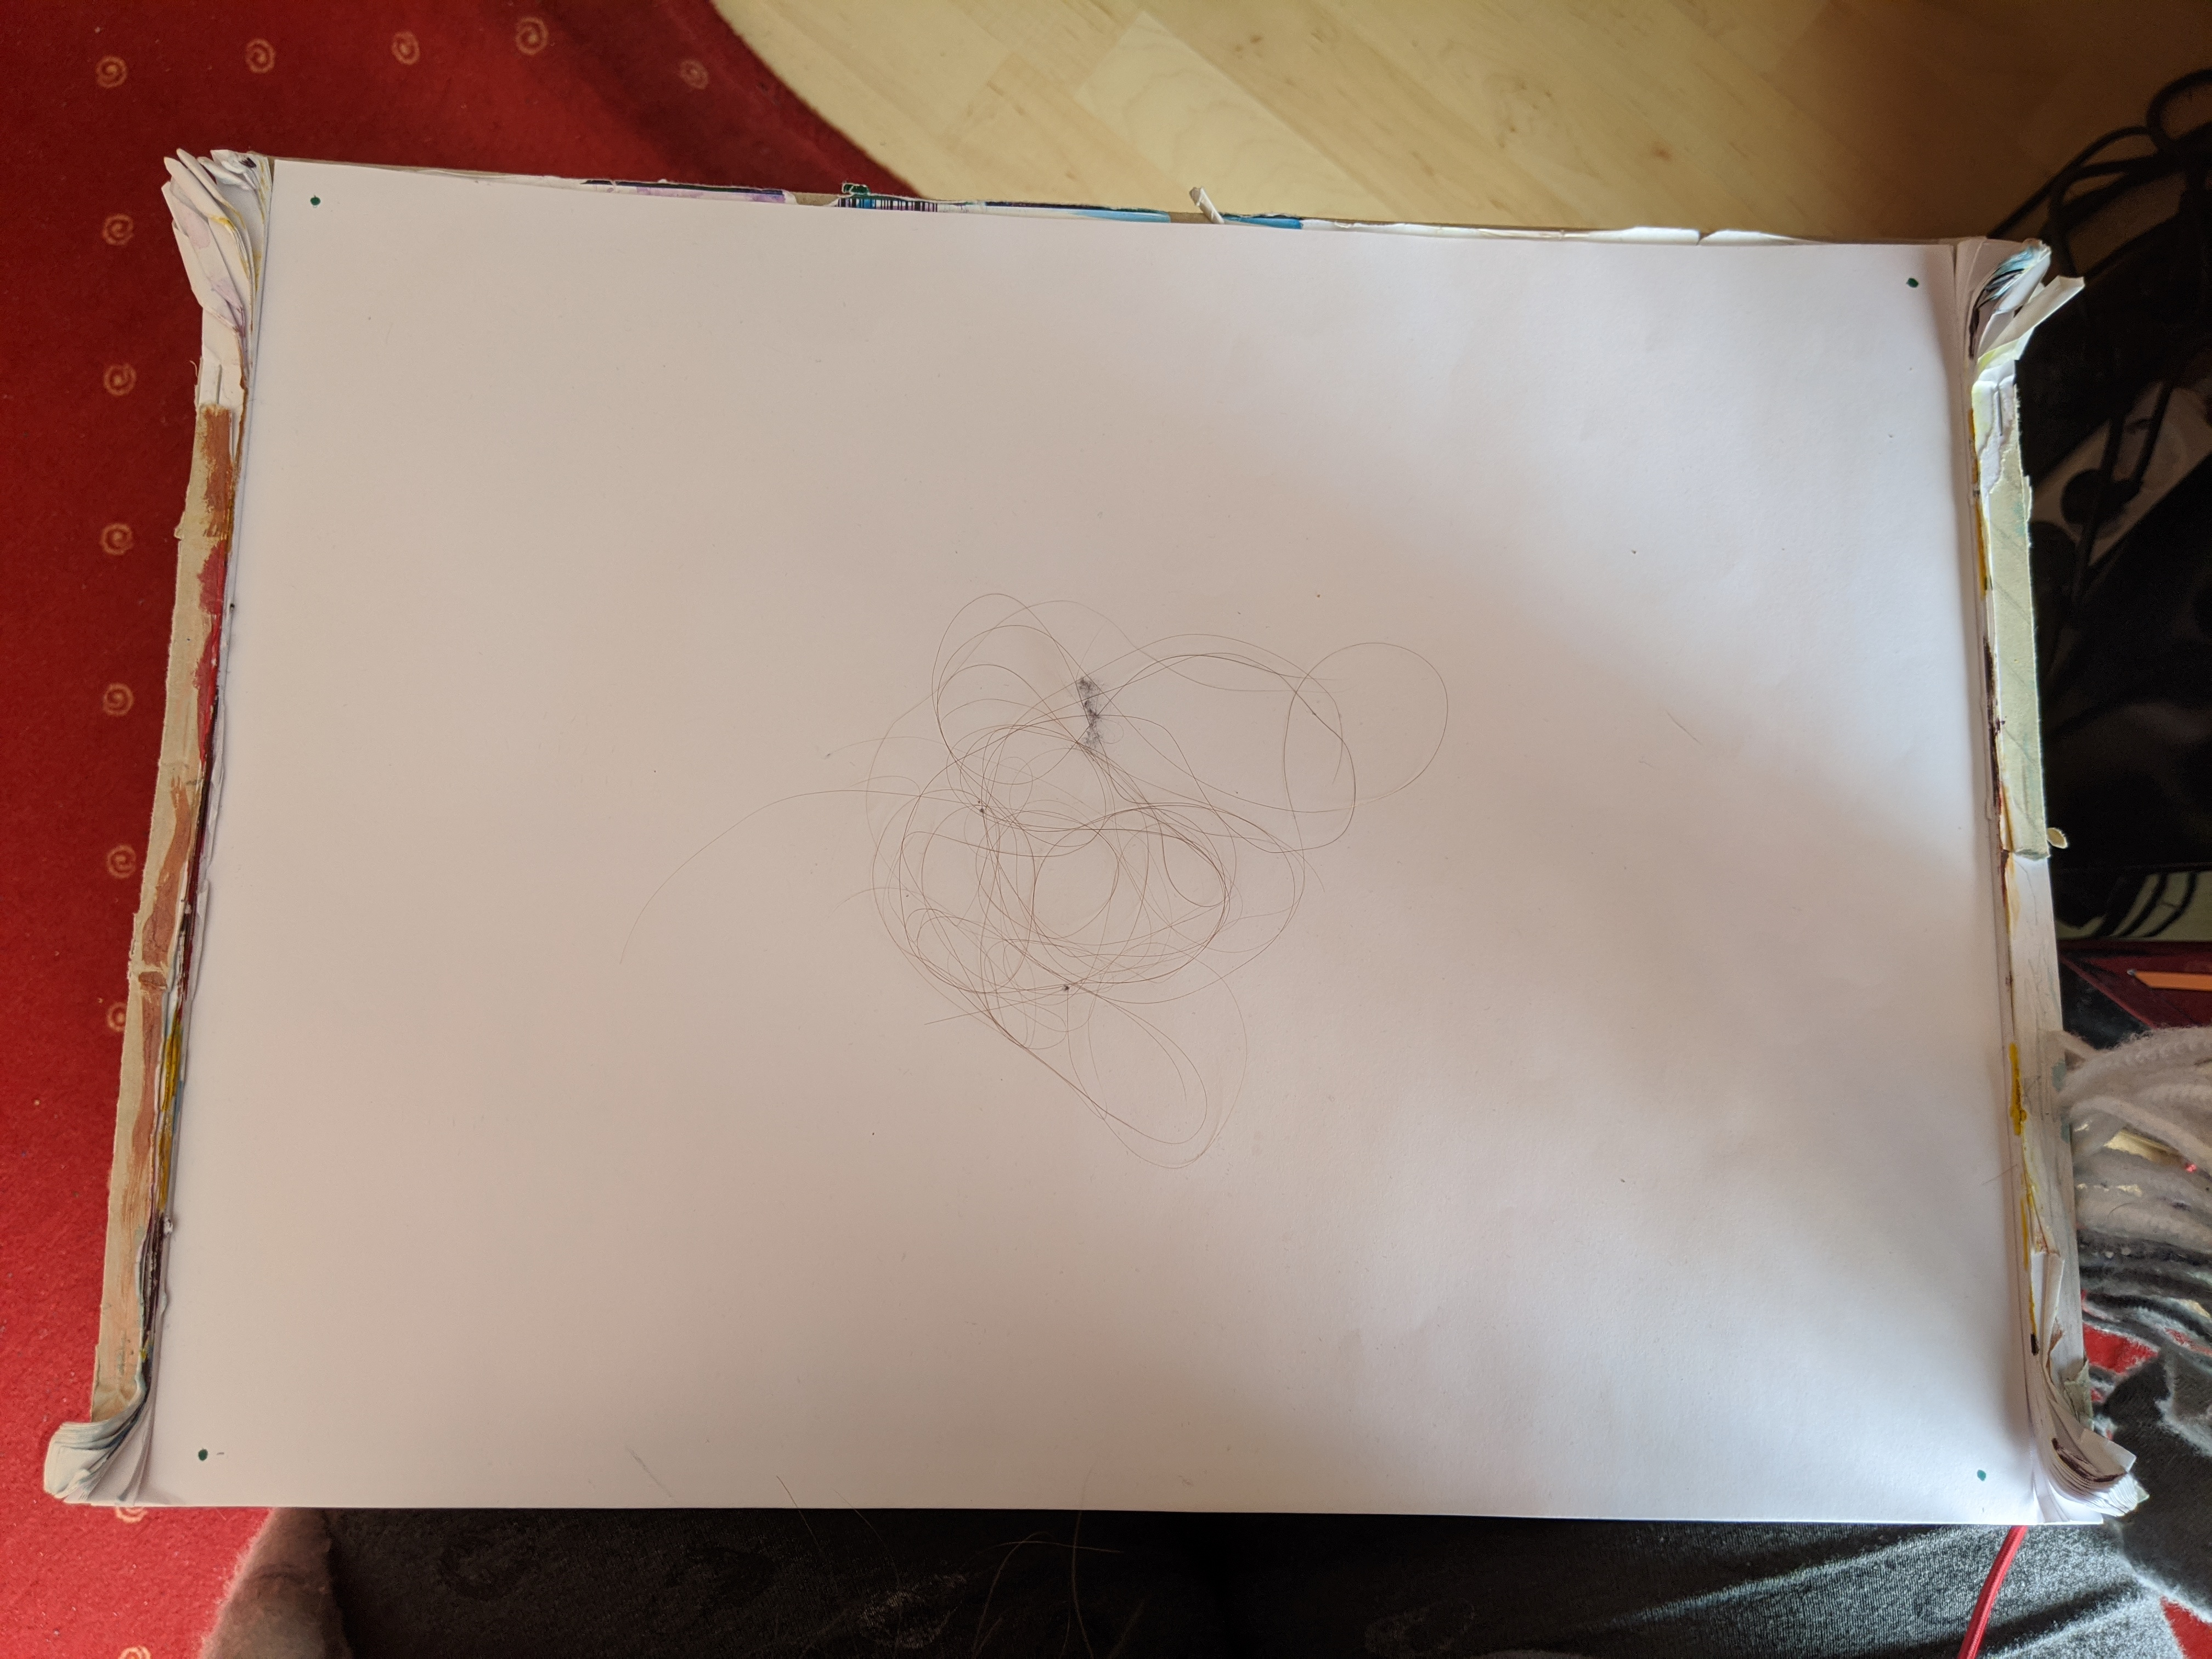
\includegraphics[width=0.6\textwidth]{fig64/00IMG_20200406_153354_12_g_15.jpg}
	\caption[]{Input}
	\label{img:input}
\end{figure}

Im ersten Schritt der Bildverarbeitung wird das Bild auf die Markierungen in den Ecken zugeschnitten. Das ist in der Methode cropDots implementiert.
Über einen Aufruf der Open CV methode matchTemplate wird nach vorkommen der Markierung gesucht. Das Resultat ist ein Karte an Wahrscheinlichkeiten, die für jedes Pixel angibt, zu welcher Wahrscheinlichkeit sich dort die Markierung befindet. Die 4 Stellen an denen die Wahrscheinlichkeit am höchsten ist, werden als Eckpunkte angesehen. Siehe Abbildung \ref{img:cropDots}.\cite{TemplateMatchingCV} 
\begin{figure*}
	\centering
	\begin{subfigure}[b]{0.475\textwidth}   
		\centering
		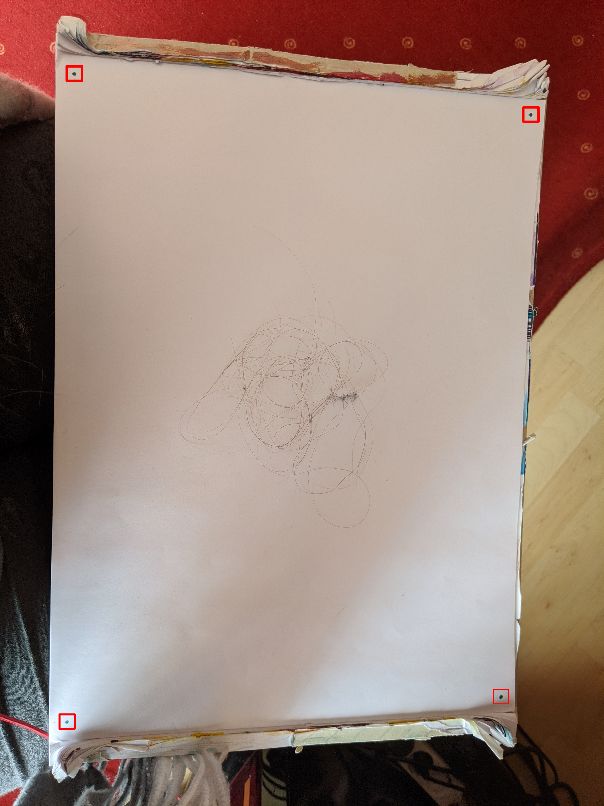
\includegraphics[width=\textwidth]{fig64/03rectImg.png}
		\caption[]{Die 4 erkannten Markierungen im Bild}
		\label{img:foundDots}
	\end{subfigure}
	\quad
	\begin{subfigure}[b]{0.475\textwidth}   
		\centering
		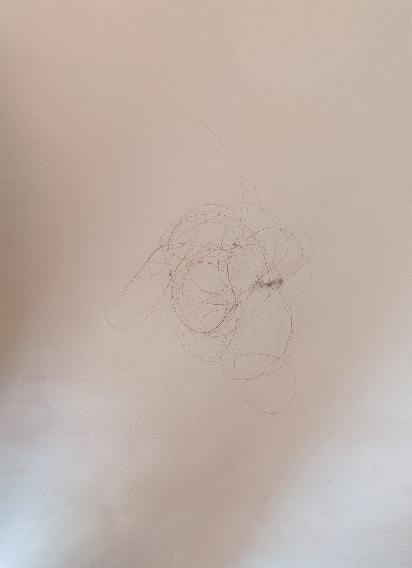
\includegraphics[width=0.9\textwidth]{fig64/03crop image.png}
		\caption[]{Resultat des Zuschneidens}
		\label{img:Crop}
	\end{subfigure}
	\caption[ der Prozess des Zuschneidens auf Markierungen in den Ecken ]
	{\small Der Prozess des Zuschneidens auf Markierungen in den Ecken} 
	\label{img:cropDots}
\end{figure*}


Durch das Zuschneiden der Bilder wird sichergestellt, das die Haare immer etwa einen gleichgroßen Hintergrund haben. So werden die Daten, die aus den Bildern gezogen werden, nicht dadurch verfälscht, das die Haare eventuell von unterschiedlichen Abständen fotografiert wurden. 

Nach dem Zuschneiden werden die Haare von dem Hintergrund getrennt.
Das ist in der Methode edgeProcess implementiert. 
Mithilfe von Canny Edge detection werden die Haare grob erkannt.
Weiße Pixel gelten als Haare, schwarze als Hintergrund. Siehe Abbildung \ref{img:Edges}.\cite{Canny}
\begin{figure*}
	\centering
	\begin{subfigure}[b]{0.475\textwidth}
		\centering
		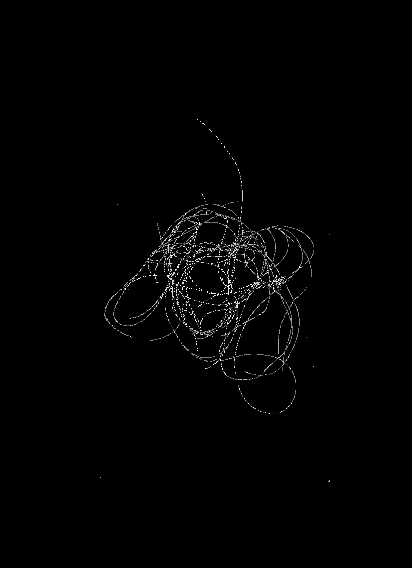
\includegraphics[width=\textwidth]{fig64/04edges.png}
		\caption[]{Canny Kantendetektion}
		\label{img:Edges} 
	\end{subfigure}
	\hfill
	\begin{subfigure}[b]{0.475\textwidth} 
		\centering
		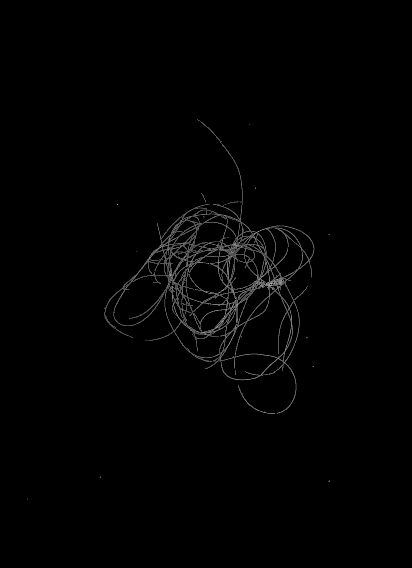
\includegraphics[width=\textwidth]{fig64/05intenstiy.png}
		\caption[]{Intensität-Abbildung der Haare}
		\label{img:Intensity}
	\end{subfigure}
	\caption[  ]
	{\small Beispiel input von knielangen dunkelroten Haare} 
	\label{img:cannywrap}
\end{figure*}


In der Methode hairPixelIntensity wird die Detektion verfeinert.
Auf das Resultat der Kantendetektion wird eine Dilatation ausgeführt. Dadurch gelten mehr Pixel als Haare und eventuelle Löcher wachsen zusammen.\cite{DilationCV}

Da Haare halb-transparent sind, wird ihre Farbe intensiver, wenn sie sich überlagern. Sie weisen eine höhere Intensität auf.
Um die Haar-Intensität zu extrahieren, wird ein Bild gebaut, in dem Hintergrund Pixel weiß sind, und Haarpixel ihren Graustufenwert aus dem Original Bild erhalten.

Sind die Haare heller als der Hintergrund, wenn es sich beispielsweise um blondes Haar auf schwarzem Hintergrund handeln, haben die Haare eine Höhere Intensität, wenn sie heller sind. Bei dunklem Haar auf hellem Hintergrund ist es gegenteilig. Die Intensität ist höher, wenn das Haar dunkler ist.
Damit beide Konstellationen zu einem ähnlichen Ergebnis kommen, werden die Graustufen invertiert, wenn die Haare hell sind. So ist auch bei ursprünglich hellem Haar, die Intensität höher, wenn die Graustufen dunkler sind.


Invertiert man das Resultat der dunkeln Haar-Intensität auf weißem Hintergrund, ergibt sich ein Bild mit schwarzem Hintergrund und Haaren, die heller sind an Stellen wo sie sich Überlagern. Siehe Abbildung \ref{img:Intensity}. Dieses Bild nennen wir Intensität-Bild.

Bevor die Intensität von dem Intensität-Bild abgelesen wird, werden Fehler in der Haar Detektion entfernt.

Die Kantendetektion erkennt oft kleine vereinzelnde Gebiete im Hintergrund. Diese Gebiete werden als Haare gewertet, auch wenn sie es nicht sind. 
Um diese Gebiete zu erkennen und zu entfernen, wird der Watershed Algorithmus angewendet. Dabei werden Marker in alle verbundenen Gebiete gesetzt, die nicht schwarz sind. Der Watershed Algorithmus lässt die Regionen wachsen. Dann werden die Regionen entfernt, die im Verglich zu der Größe des Bildes sehr klein sind. Siehe Abbildung \ref{img:smallRegionwrap}. \cite{Watershed,WatershedCV,ConnectedComponents}

Die Summe aller Graustufenwerte des bereinigten Intensität-Bildes wird als Intensität gespeichert. Dabei wird der Hintergrund außer Acht gelassen, weil es schwarz ist, und somit den Graustufenwert 0 hat.
\begin{figure*}
	\centering
	\begin{subfigure}[b]{0.475\textwidth}
		\centering
		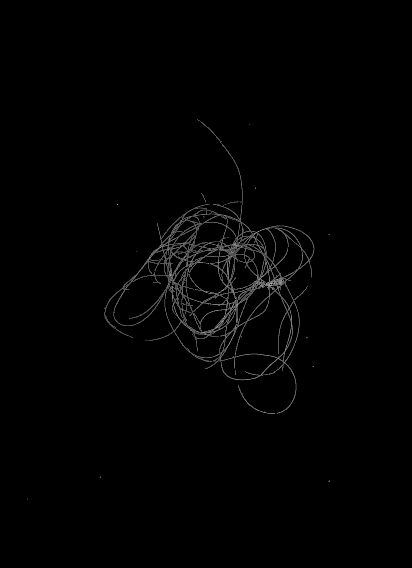
\includegraphics[width=\textwidth]{fig64/05intenstiy.png}
		\caption[]{Intensität-Abbildung der Haare}
		\label{img:Intensity2}
	\end{subfigure}
	\hfill
	\begin{subfigure}[b]{0.475\textwidth} 
		\centering
		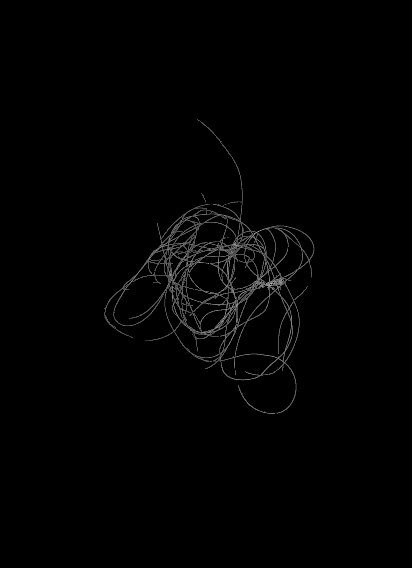
\includegraphics[width=\textwidth]{fig64/06small regions removed.png}
		\caption[]{Kleine Regionen Entfernt}
		\label{img:smallRegion}
	\end{subfigure}
	\caption[  ]
	{\small Enternen von kleinen Regionen, vorher nachher} 
	\label{img:smallRegionwrap}
\end{figure*}

In der Methode hairPixelPercentage werden die Pixel gezählt die als Haare gelten. Zusätzlich wird der Prozentsatz an Haar Pixeln und die Intensität des Bildes im Vergleich zur Bildgröße gespeichert. 

Dann wird die Dichte der Haare in der Methode backgroundRegions Untersucht.
Dafür werden mithilfe von Watershed die Hintergrund Regionen bestimmt, die durch Haare getrennt werden.
Die Marker werden in alle zusammenhängenden Hintergrundgebiete gesetzt.\cite{Watershed,WatershedCV}

Die Größe der Region, die die Haare umschließt wird gespeichert. Abbildung \ref{img:outerSection}.
Zusätzlich wird die Anzahl der Regionen, die von Haaren umschlossen werden und deren Durchschnittliche Größe, gespeichert.\cite{Watershed,WatershedCV}
\begin{figure*}
	\centering
	\begin{subfigure}[b]{0.475\textwidth}
		\centering
		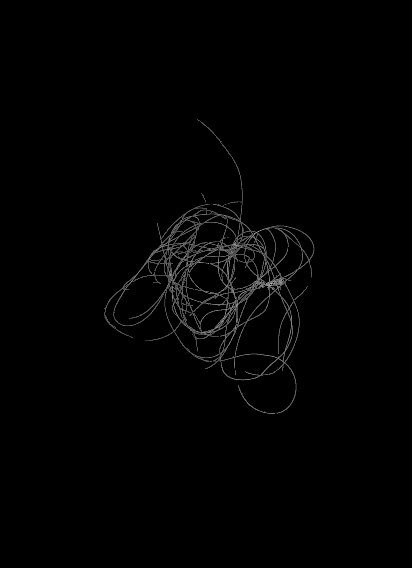
\includegraphics[width=\textwidth]{fig64/06small regions removed.png}
		\caption[]{watershed input}
		\label{img:wsiput}
	\end{subfigure}
	\hfill
	\begin{subfigure}[b]{0.475\textwidth} 
		\centering
		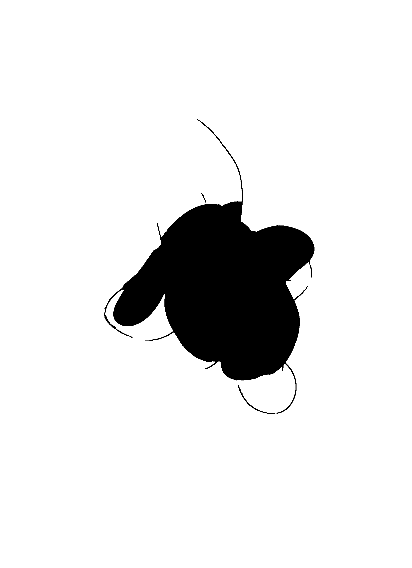
\includegraphics[width=\textwidth]{fig64/08outer section.png}
		\caption[]{Äußere Region isoliert und in weiß dargestellt.}
		\label{img:outerSection}
	\end{subfigure}
	\caption[  ]
	{\small Anwendung von Watershed} 
	\label{img:regionwrap}
\end{figure*}

Als nächstes werden die Gebiete des Bildes untersucht, die eine erhöhte Haar-Dichte aufweisen.
Dafür wird das Intensität-Bild skelettiert. Siehe Abbildung \ref{img:skel}.
Die Hintergrund Regionen werden wie zuvor untersucht.

\begin{figure*}
	\centering
	\begin{subfigure}[b]{0.475\textwidth}
		\centering
		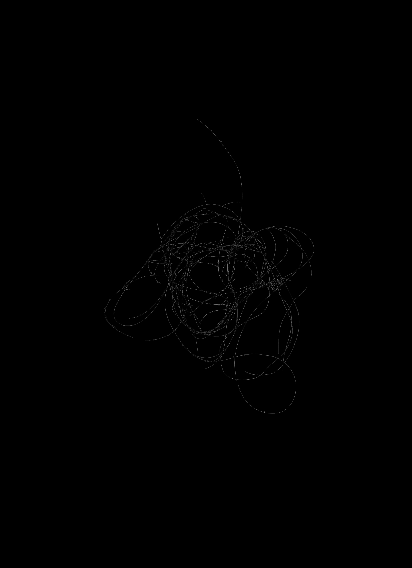
\includegraphics[width=\textwidth]{fig64/09input intensity.png}
		\caption[]{Skelett des Intensität-Bildes}
		\label{img:skel}
	\end{subfigure}
	\hfill
	\begin{subfigure}[b]{0.475\textwidth} 
		\centering
		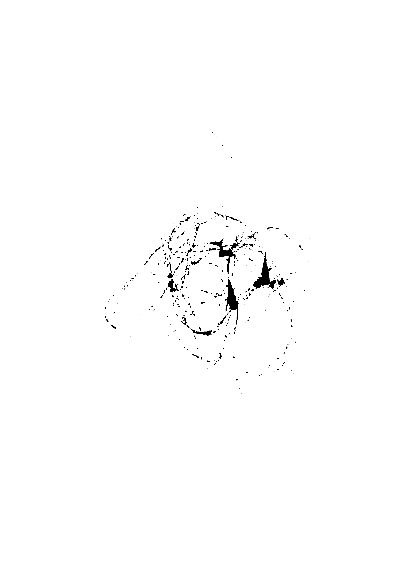
\includegraphics[width=\textwidth]{fig64/09outer section.png}
		\caption[]{Äußerte Region des skelettierten Bildes}
		\label{img:skelBGregion}
	\end{subfigure}
	\caption[  ]
	{\small Dichtere Regionen untersuchen} 
	\label{img:skelwarp}
\end{figure*}

In der Methode denseAndLoosePerc wird die Haar-Intensität in den dichteren Regionen und in den weniger dichten Regionen berechnet und abgespeichert.

Bei einem Durchlauf von detect wird für ein Bild insgesamt 28 Datenpunkte extrahiert und abgespeichert. Siehe Anhang \ref{appendix:datenpunkte}. 



\subsection{Kalibrieren}

Die Kalibrierung ist in der Methode calibration implementiert.
Es werden mehrere Bilder als Input angegeben. Für jedes der Bilder wird die Menge der Haare in dem Titel des Bildes übergeben. 
Die Bilder werden alle mit detect Untersucht. Die Daten aus den Untersuchungen, sowie die Haar-Mengen werden abgespeichert.

\subsection{Schätzen eines Haar-Bildes}

Nachdem eine Kalibrierung durchgeführt wurde, kann die Haar-Anzahl auf beliebigen Bildern geschätzt werden.
Das Schätzen ist in der Methode readFilesAndGuess implementiert.

Zuerst wird das zu schätzende Bild, mithilfe von detect, untersucht.
Dann werden die Daten aus der Kalibrierung geladen. 
Die Daten werden teilweise miteinander verrechnet und dann auf die dazugehörigen Haar-Anzahlen abgebildet.
So entsteht eine Menge an Graphen, bei denen die Haar-Anzahl jeweils auf der y Achse liegt. Siehe Abbildung \ref{fig:mapping}. 

\begin{figure}
	\centering
	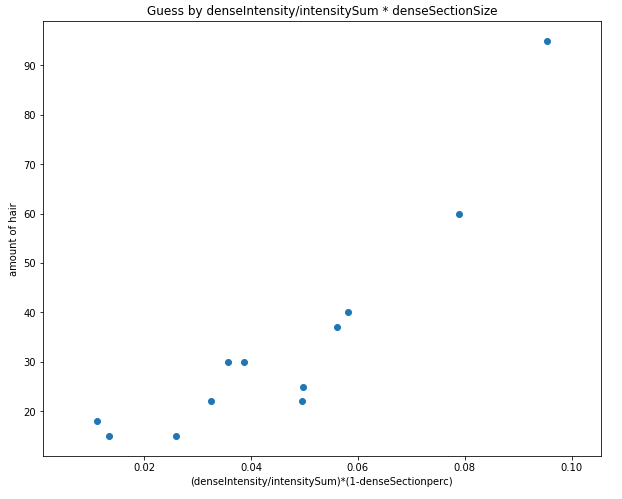
\includegraphics[width=0.8\textwidth]{fig64/gh4.PNG}
	\caption[]{Haar-Anzahl in Relation zur Intensität in dichten Regionen normalisiert durch gesamte Intensität und Region-Größe}
	\label{fig:mapping}
\end{figure}

Die Punkte in den Graphen werden durch jeweils 3 Funktionen Approximiert. Eine Lineare Regression, eine Spline-Interpolation, und eine benutzerdefinierte Fitted Curve.
Der Benutzer kann aus linear, logarithmisch und exponentiell aussuchen.
Siehe Abbildung \ref{fig:func}.

\begin{figure}
	\centering
	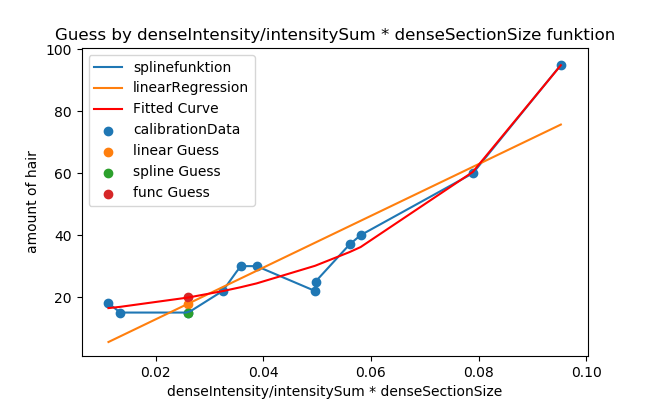
\includegraphics[width=0.9\textwidth]{fig64/g11_denseIntensitynormDetailed.png}
	\caption[]{Funktionen, die Datenpunkte Approximieren. Spline-Interpolation, lineare Regression und exponentielle Funktion.}
	\label{fig:func}
\end{figure} 

Von den 28 Datenpunkten die aus den Bildern ausgewertet werden, werden 17 Genutzt um 12 Modelle zu erstellt. Diese Modelle wurden als aussagekräftig befunden, um Haar-Anzahlen schätzen zu können. Untersucht werden die Menge der Pixel, die als Haare zählen, sowie die Intensität und die Größe und Anzahl der Hintergrund-Regionen. Siehe Anhang \ref{appendix:xwertemodel} Für die Berechnungen der genutzten x Werte für die Modelle. 

Siehe den Anhang \ref{appendix:modelle} für die graphische Darstellung der Modelle.

Für jedes der Modelle werden 3 Funktionen approximiert. Mit den Funktionen werden jeweils 3 Schätzungen für das zu schätzende Bild berechnet. 

Dabei kann es zu Ausreißern kommen. Alle Schätzungen von weniger als 0 Haaren werden entfernt und statistische Ausreißer werden mithilfe eines Algorithmus basierend auf dem Tschebyscheff Theorem entfernt.\cite{outlierRemoval}

Der Mittelwert, der übrig gebliebenen Schätzungen, ist das Endergebnis. 
Siehe Anhang \ref{appendix:komm}.
\subsection*{Tests}
\subsection{Test: Knielange, dunkelrote Haare}

Diese Haare wurden auf einem weißem Hintergrund aufgenommen. Die Ecken wurden mit dunkeln Punkten markiert. Siehe Abbildung \ref{img:tstM}.

\begin{figure*}
	\centering
	\begin{subfigure}[b]{0.475\textwidth}
		\centering
		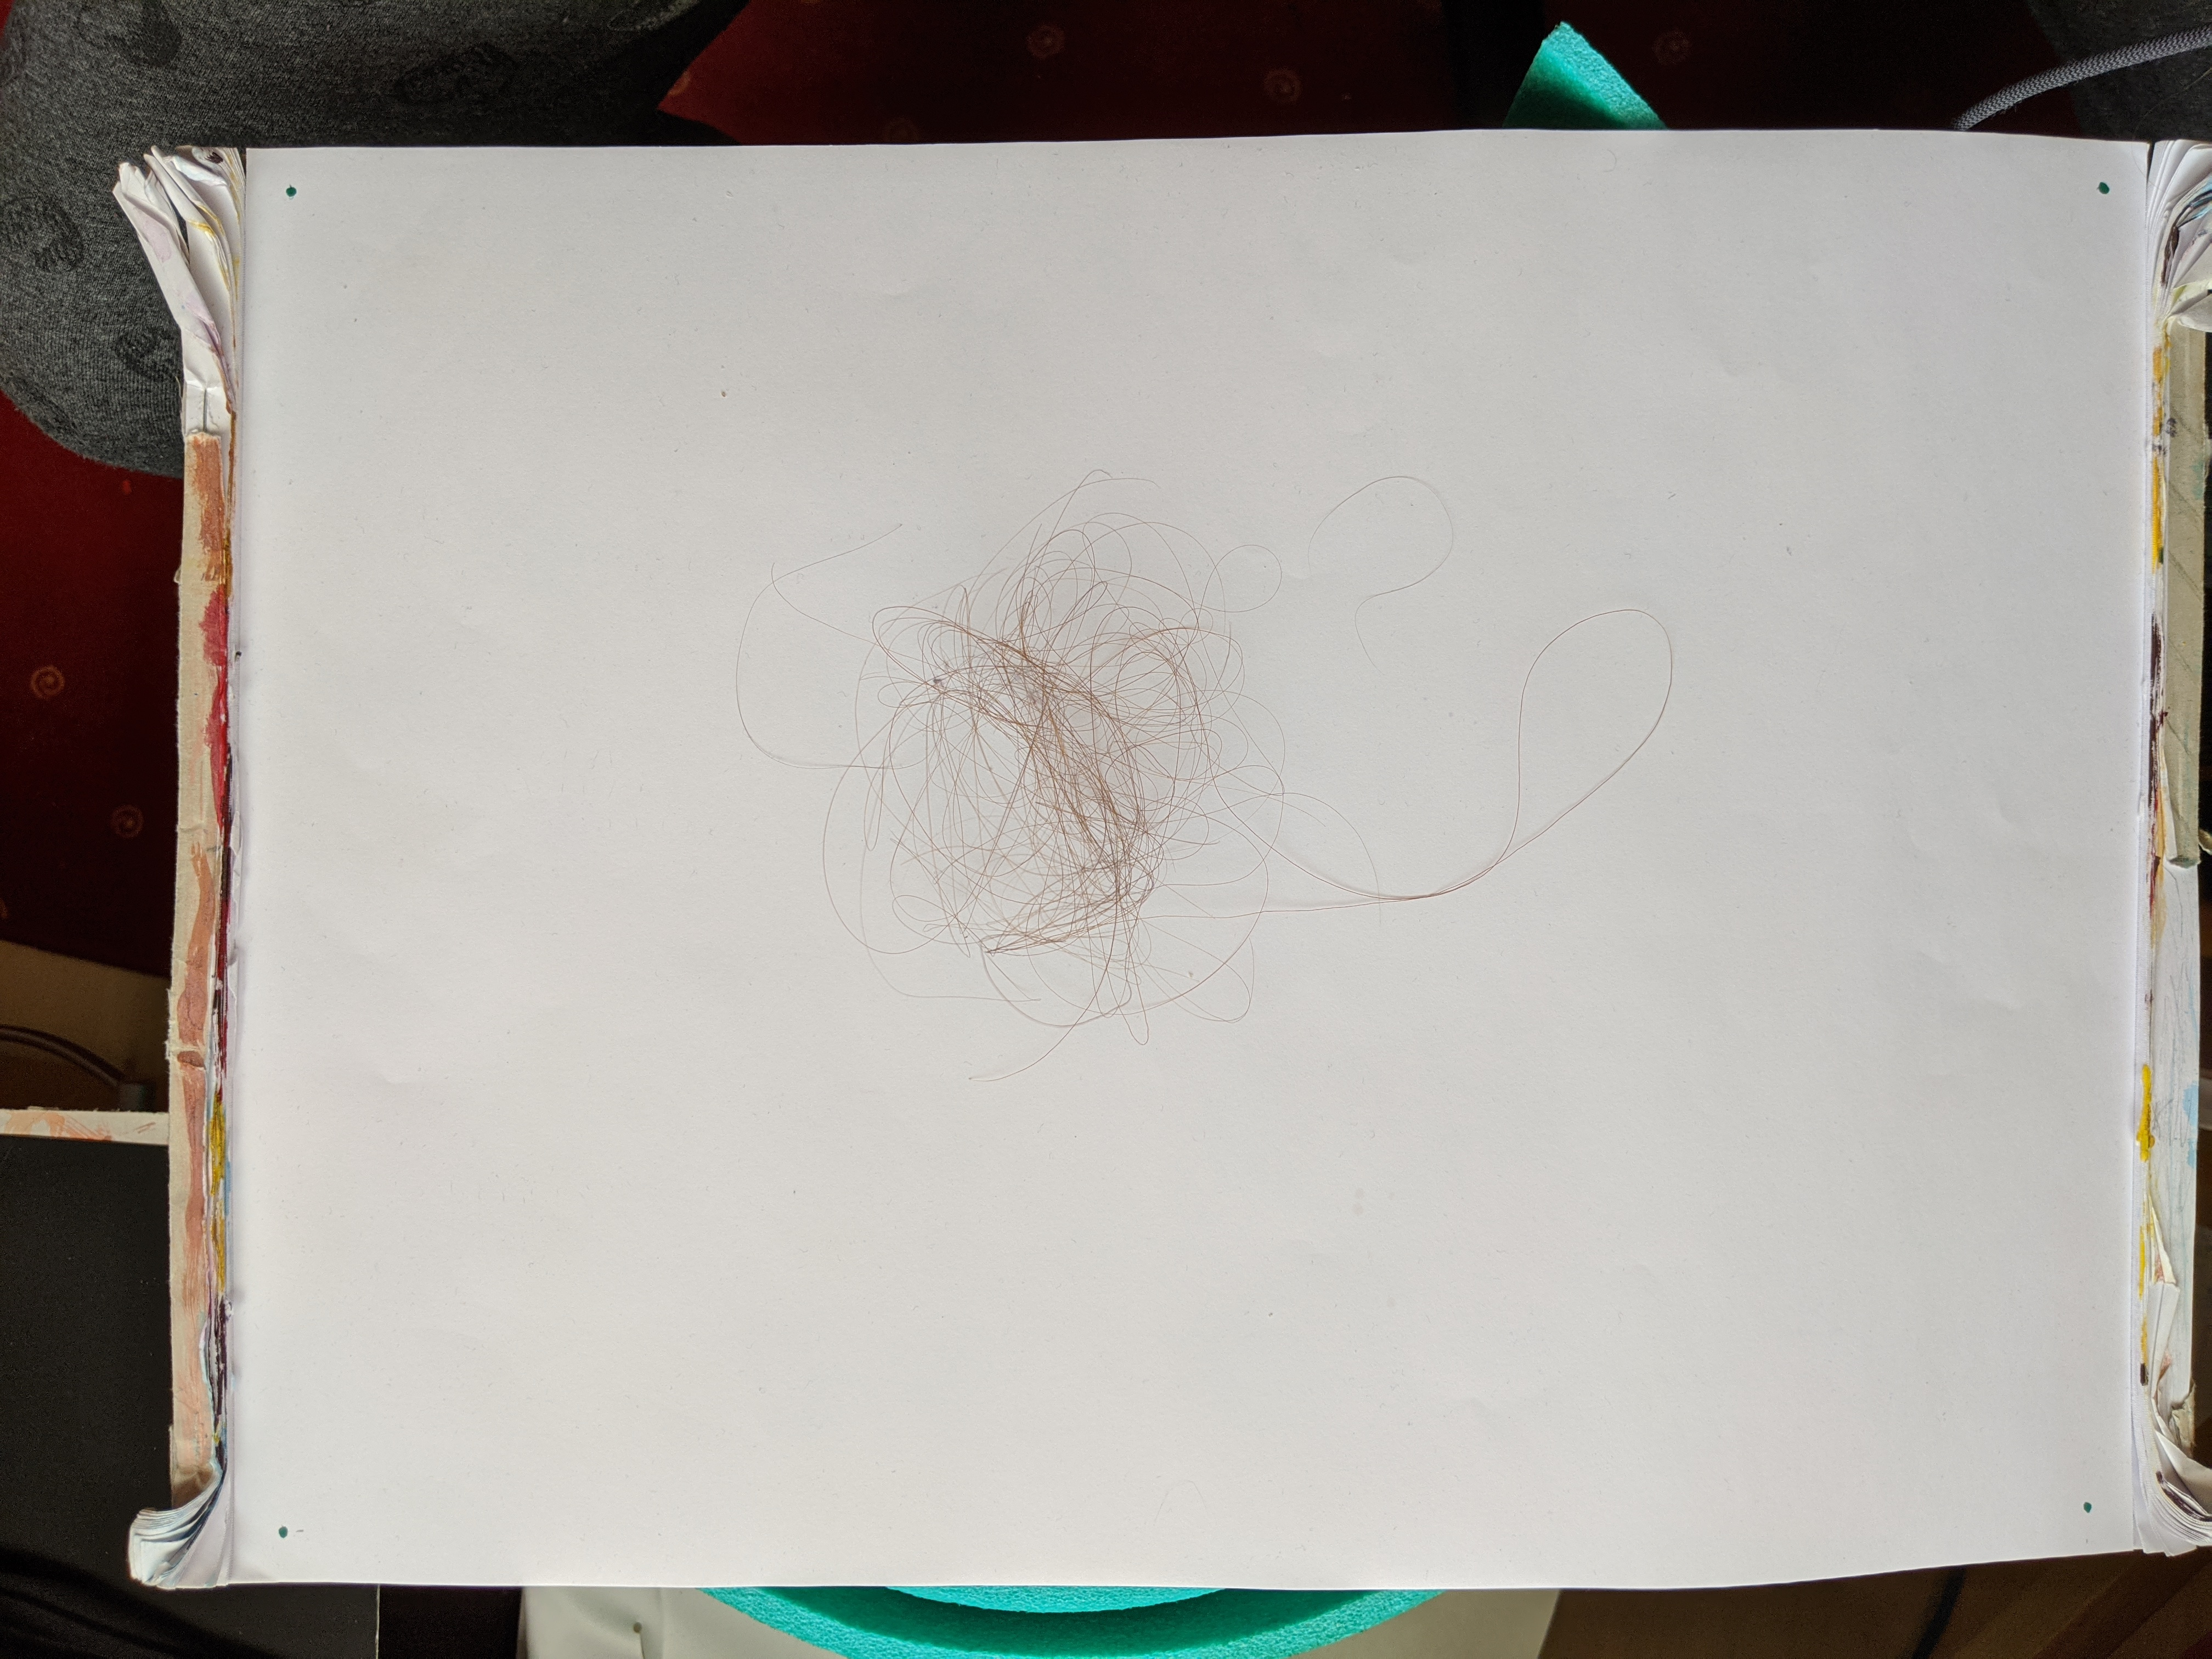
\includegraphics[width=\textwidth]{figMummel/IMG_20200325_172536_30.jpg}
		\caption[]{Geschätzt auf 27 Haare. Tatsächlich 30 Haare}
		\label{img:tstM1} 
	\end{subfigure}
	\hfill
	\begin{subfigure}[b]{0.475\textwidth} 
		\centering
		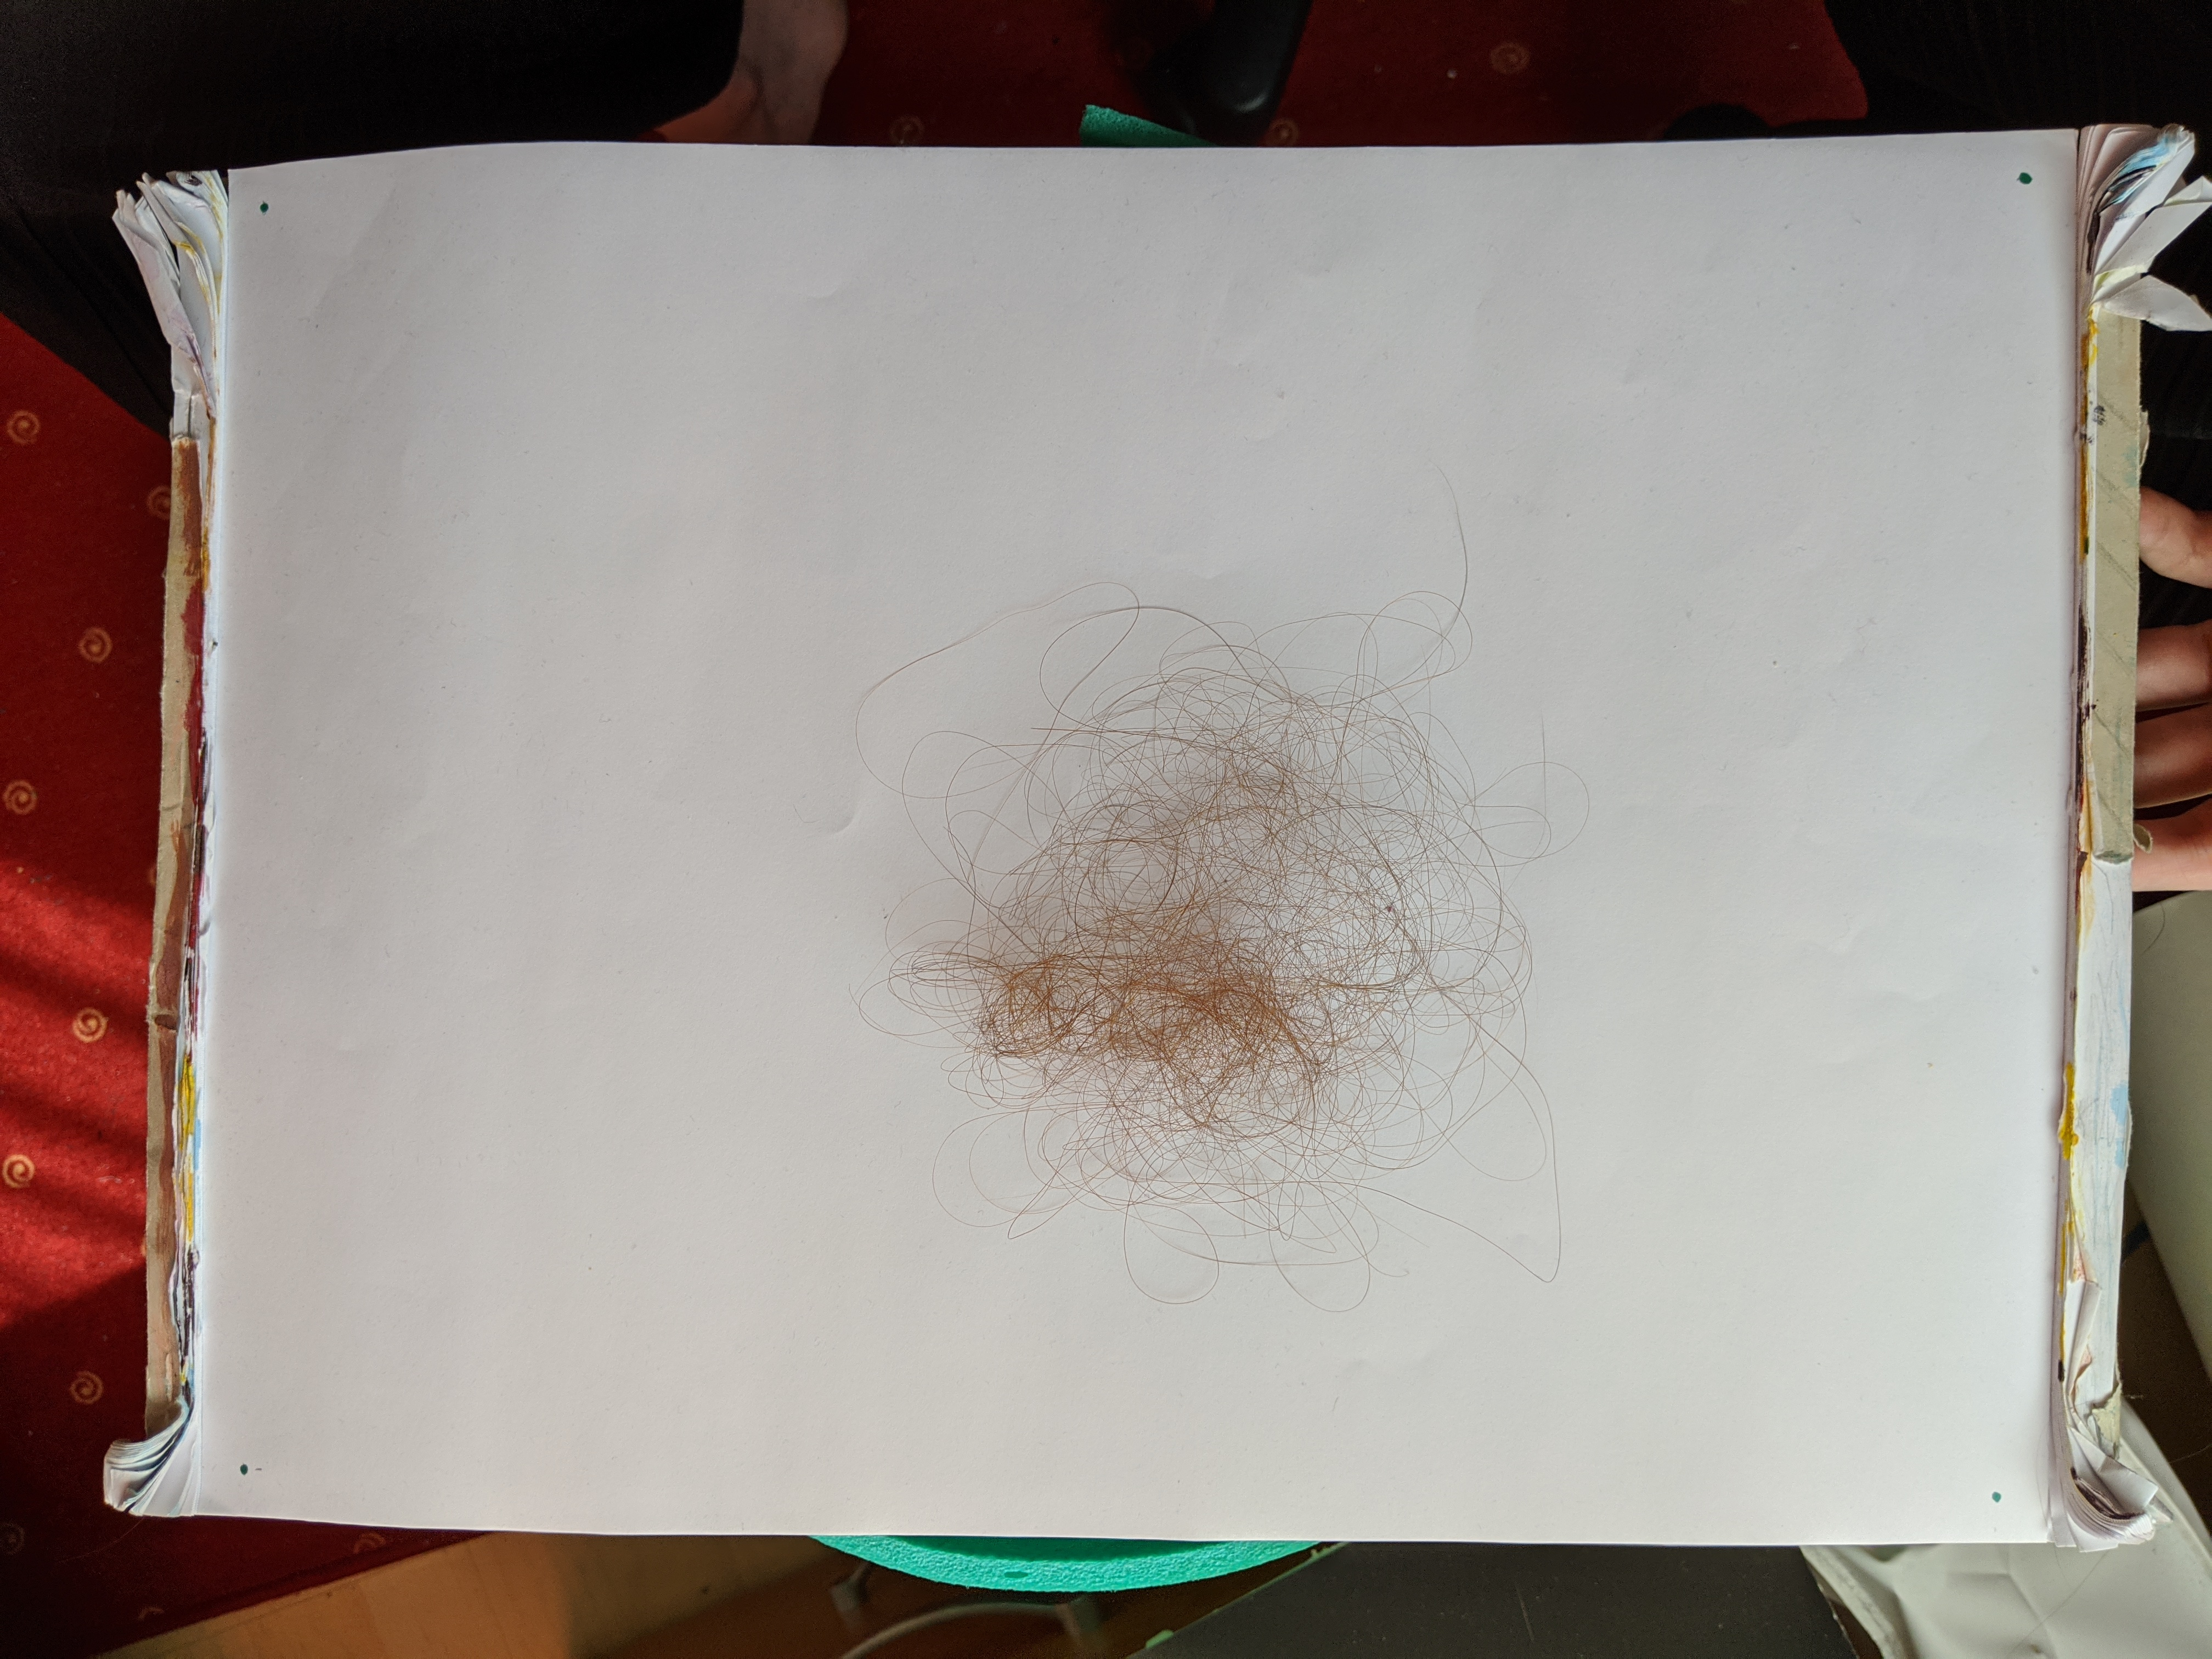
\includegraphics[width=\textwidth]{figMummel/IMG_20200327_132125_95.jpg}
		\caption[]{Geschätzt auf 89 Haare. Tatsächlich 95.}
		\label{img:tstM2}
	\end{subfigure}
	\caption[  ]
	{\small Beispiel input von dunkelroten langen Haaren} 
	\label{img:tstM}
\end{figure*}

Es wurde eine Untersuchung in einem Zeitraum von 7 Wochen von dem tägliche Haarausfall angestellt. Siehe Abbildung \ref{img:7weeks}.
\begin{figure}
	\centering
	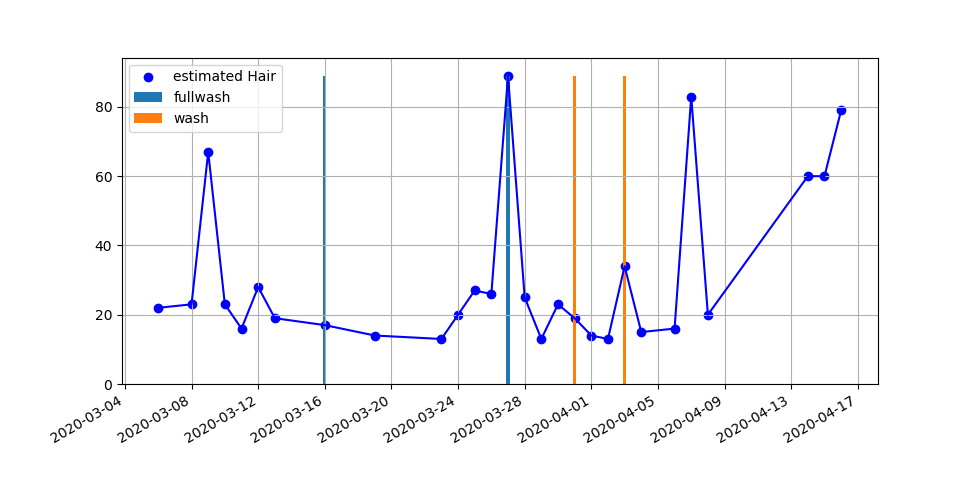
\includegraphics[width=.9\textwidth]{fig64/plot.png}
	\caption[]{Schätzungen aus einem Zeitraum von 7 Wochen}
	\label{img:7weeks}
\end{figure} 

Um die Fehlerrate testen zu können, wurde für die Input Bilder die Anzahl der Haare per Hand gezählt.
Die Differenz zwischen der tatsächlicher Haaranzahl und der geschätzter Haaranzahl gilt als Fehler pro Schätzung. Der durchschnittliche Fehler, ist die Anzahl an Haaren, um die sich das Programm im Durchschnitt verschätzt. 

Mit 12 Kalibration-Bildern, wurden 27 Schätzungen durchgeführt. Es kam zu einem durchschnittlichen Fehler von 5.03 Haaren.
Der Größte Error liegt bei 16 Haaren. Der niedrigste bei 0. 

Mit einer kleineren Kalibrations-Menge 3 Bildern wurde ein durchschnittlicher Fehler von 6.8 Haare über 27 Schätzungen gefunden. Auch hier liegt der Höchste Fehler bei 16 und der niedrigste bei 0. Siehe Anhang \ref{appendix:Error}.

Bei einem beispielhaften Durchlauf der Bildverarbeitung, dauerte der Prozess 34 Sekunden. 94\% der Zeit wurden dabei verbraucht, die Regionen des Bildes durchzugehen, um kleine Regionen zu entfernen und die Größe von Hintergrundregionen festzuhalten.

\begin{lstlisting}[style=DOS]
guessing the amount of hair in the picture
started processing at 2020-04-24 18:41:52.549785
image path Users/Mummel/estimationInput/
IMG_20200417_154758_2days.jpg
cropping image to TemplateDot using PatternMatching
Users/Mummel
2020-04-24 18:41:53.341533 elapsed time 0:00:00.791748
2020-04-24 18:41:53.343535 elapsed time 0:00:00.002002
detecting Hair via edge detection
2020-04-24 18:41:53.363527 elapsed time 0:00:00.019992
backgroundcolor 205.49759540621406
removing smaller Regions...
looping though sections took: 0:00:02.692153
done
2020-04-24 18:41:56.322595 elapsed time 0:00:02.959068
2020-04-24 18:41:56.330593 elapsed time 0:00:00.007998
processing background regions...
innerSectionNum 621
looping though sections took: 0:00:09.474014
done
2020-04-24 18:42:06.037533 elapsed time 0:00:09.706940
skeletonize
skeletonizing took 0:00:00.291908
processing background regions...
innerSectionNum 1287
looping though sections took: 0:00:20.393568
done
2020-04-24 18:42:26.967931 elapsed time 0:00:20.930398
2020-04-24 18:42:27.058901 elapsed time 0:00:00.090970
Image Processing took : 0:00:34.509116
\end{lstlisting}

\subsection{Test: Hüftlange, feine, blonde Haare}

Blonde Haare wurden vor einem Schwarzen Hintergrund aufgenommen. Siehe Abbildung \ref{img:tstB}.

\begin{figure*}
	\centering
	\begin{subfigure}[b]{0.475\textwidth}
		\centering
		\includegraphics[width=\textwidth]{testFig/B_IMG_20200322_093659_50.jpg}
		\caption[]{Geschätzt auf 37 Haare. Tatsächlich 50 Haare}
		\label{img:tstB1} 
	\end{subfigure}
	\hfill
	\begin{subfigure}[b]{0.475\textwidth} 
		\centering
		\includegraphics[width=\textwidth]{testFig/B_IMG_20200330_094438_20.jpg}
		\caption[]{Geschätzt auf 24 Haare. Tatsächlich 20.}
		\label{img:tstB2}
	\end{subfigure}
	\caption[  ]
	{\small Beispiel input von blonden langen Haaren} 
	\label{img:tstB}
\end{figure*}
Für den schwarzen Hintergrund wurde besonders matte schwarze Pappe verwendet. Wenn die Struktur der Pappe zu grob ist, oder durch das Reflektieren von Licht sichtbar wird, wird sie von Canny Edge detection erkannt.
 
Auf schwarzem Hintergrund ist Staub besonders gut sichtbar, was zu Problemen beim Template Matching geführt hat. Der Staub wurde mit den Punkten verwechselt, die die Ecken des Bildes markieren.

Daher wurden die Markierungen zu Kreuzen geändert. Diese werden deutliche seltenen mit Staub verwechselt. 

Mit eine Kalibrations-Menge von 4 Bildern ergab sich ein durchschnittlicher Fehler von 6.9 Haaren über 20 Schätzungen. 
Siehe Anhang \ref{appendix:Error}.

Siehe Anhang \ref{appendix:Blond} für Schätzungs-Modelle und die Verarbeitung von Blonden Haaren.

Bei den Blonden Haaren dauert die Bildverarbeitung bei einem Beispiel 37 Sekunden. 
Auch hier verbrauchen Prozesse, die durch Regionen durchgehen 94\% der Zeit.

Obwohl besonders matte schwarze Pappe als Hintergrund gewählt wurde, erkennt Canny Edge detection viele Unebenheiten und Verschmutzungen. Siehe Abbildung \ref{fig:BinaRawIntensity}. Diese werden währen dem Schritt "removing smaller Regions" entfernt. Es dauert 21 Sekunden in dem Beispieldurchlauf. 

\begin{lstlisting}[style=DOS]
guessing the amount of hair in the picture
started processing at 2020-04-24 18:40:29.795237
image path Users/Bina/estimationInput/IMG_20200312_25.jpg
cropping image to TemplateDot using PatternMatching
Users/Bina
fliping image cuz it is blond
2020-04-24 18:40:31.338249 elapsed time 0:00:01.543012
2020-04-24 18:40:31.341249 elapsed time 0:00:00.003000
detecting Hair via edge detection
2020-04-24 18:40:31.357244 elapsed time 0:00:00.015995
backgroundcolor 123.07201030937907
removing smaller Regions...
looping though sections took: 0:00:21.209313
done
2020-04-24 18:40:52.807480 elapsed time 0:00:21.450236
2020-04-24 18:40:52.813479 elapsed time 0:00:00.005999
processing background regions...
innerSectionNum 328
looping though sections took: 0:00:04.352129
done
2020-04-24 18:40:57.368542 elapsed time 0:00:04.555063
skeletonize
skeletonizing took 0:00:00.214933
processing background regions...
innerSectionNum 264
looping though sections took: 0:00:03.507895
done
2020-04-24 18:41:01.301302 elapsed time 0:00:03.932760
2020-04-24 18:41:01.379277 elapsed time 0:00:00.077975
Image Processing took : 0:00:31.585040
\end{lstlisting}

\subsection{Test: Kurze, hellbraune Haare}

Für hellbraune Haare hat es sich gezeigt, das ein schwarzer Hintergrund einen besseren Kontrast bietet, als ein Weißer.

\begin{figure*}
	\centering
	\begin{subfigure}[b]{0.475\textwidth}
		\centering
		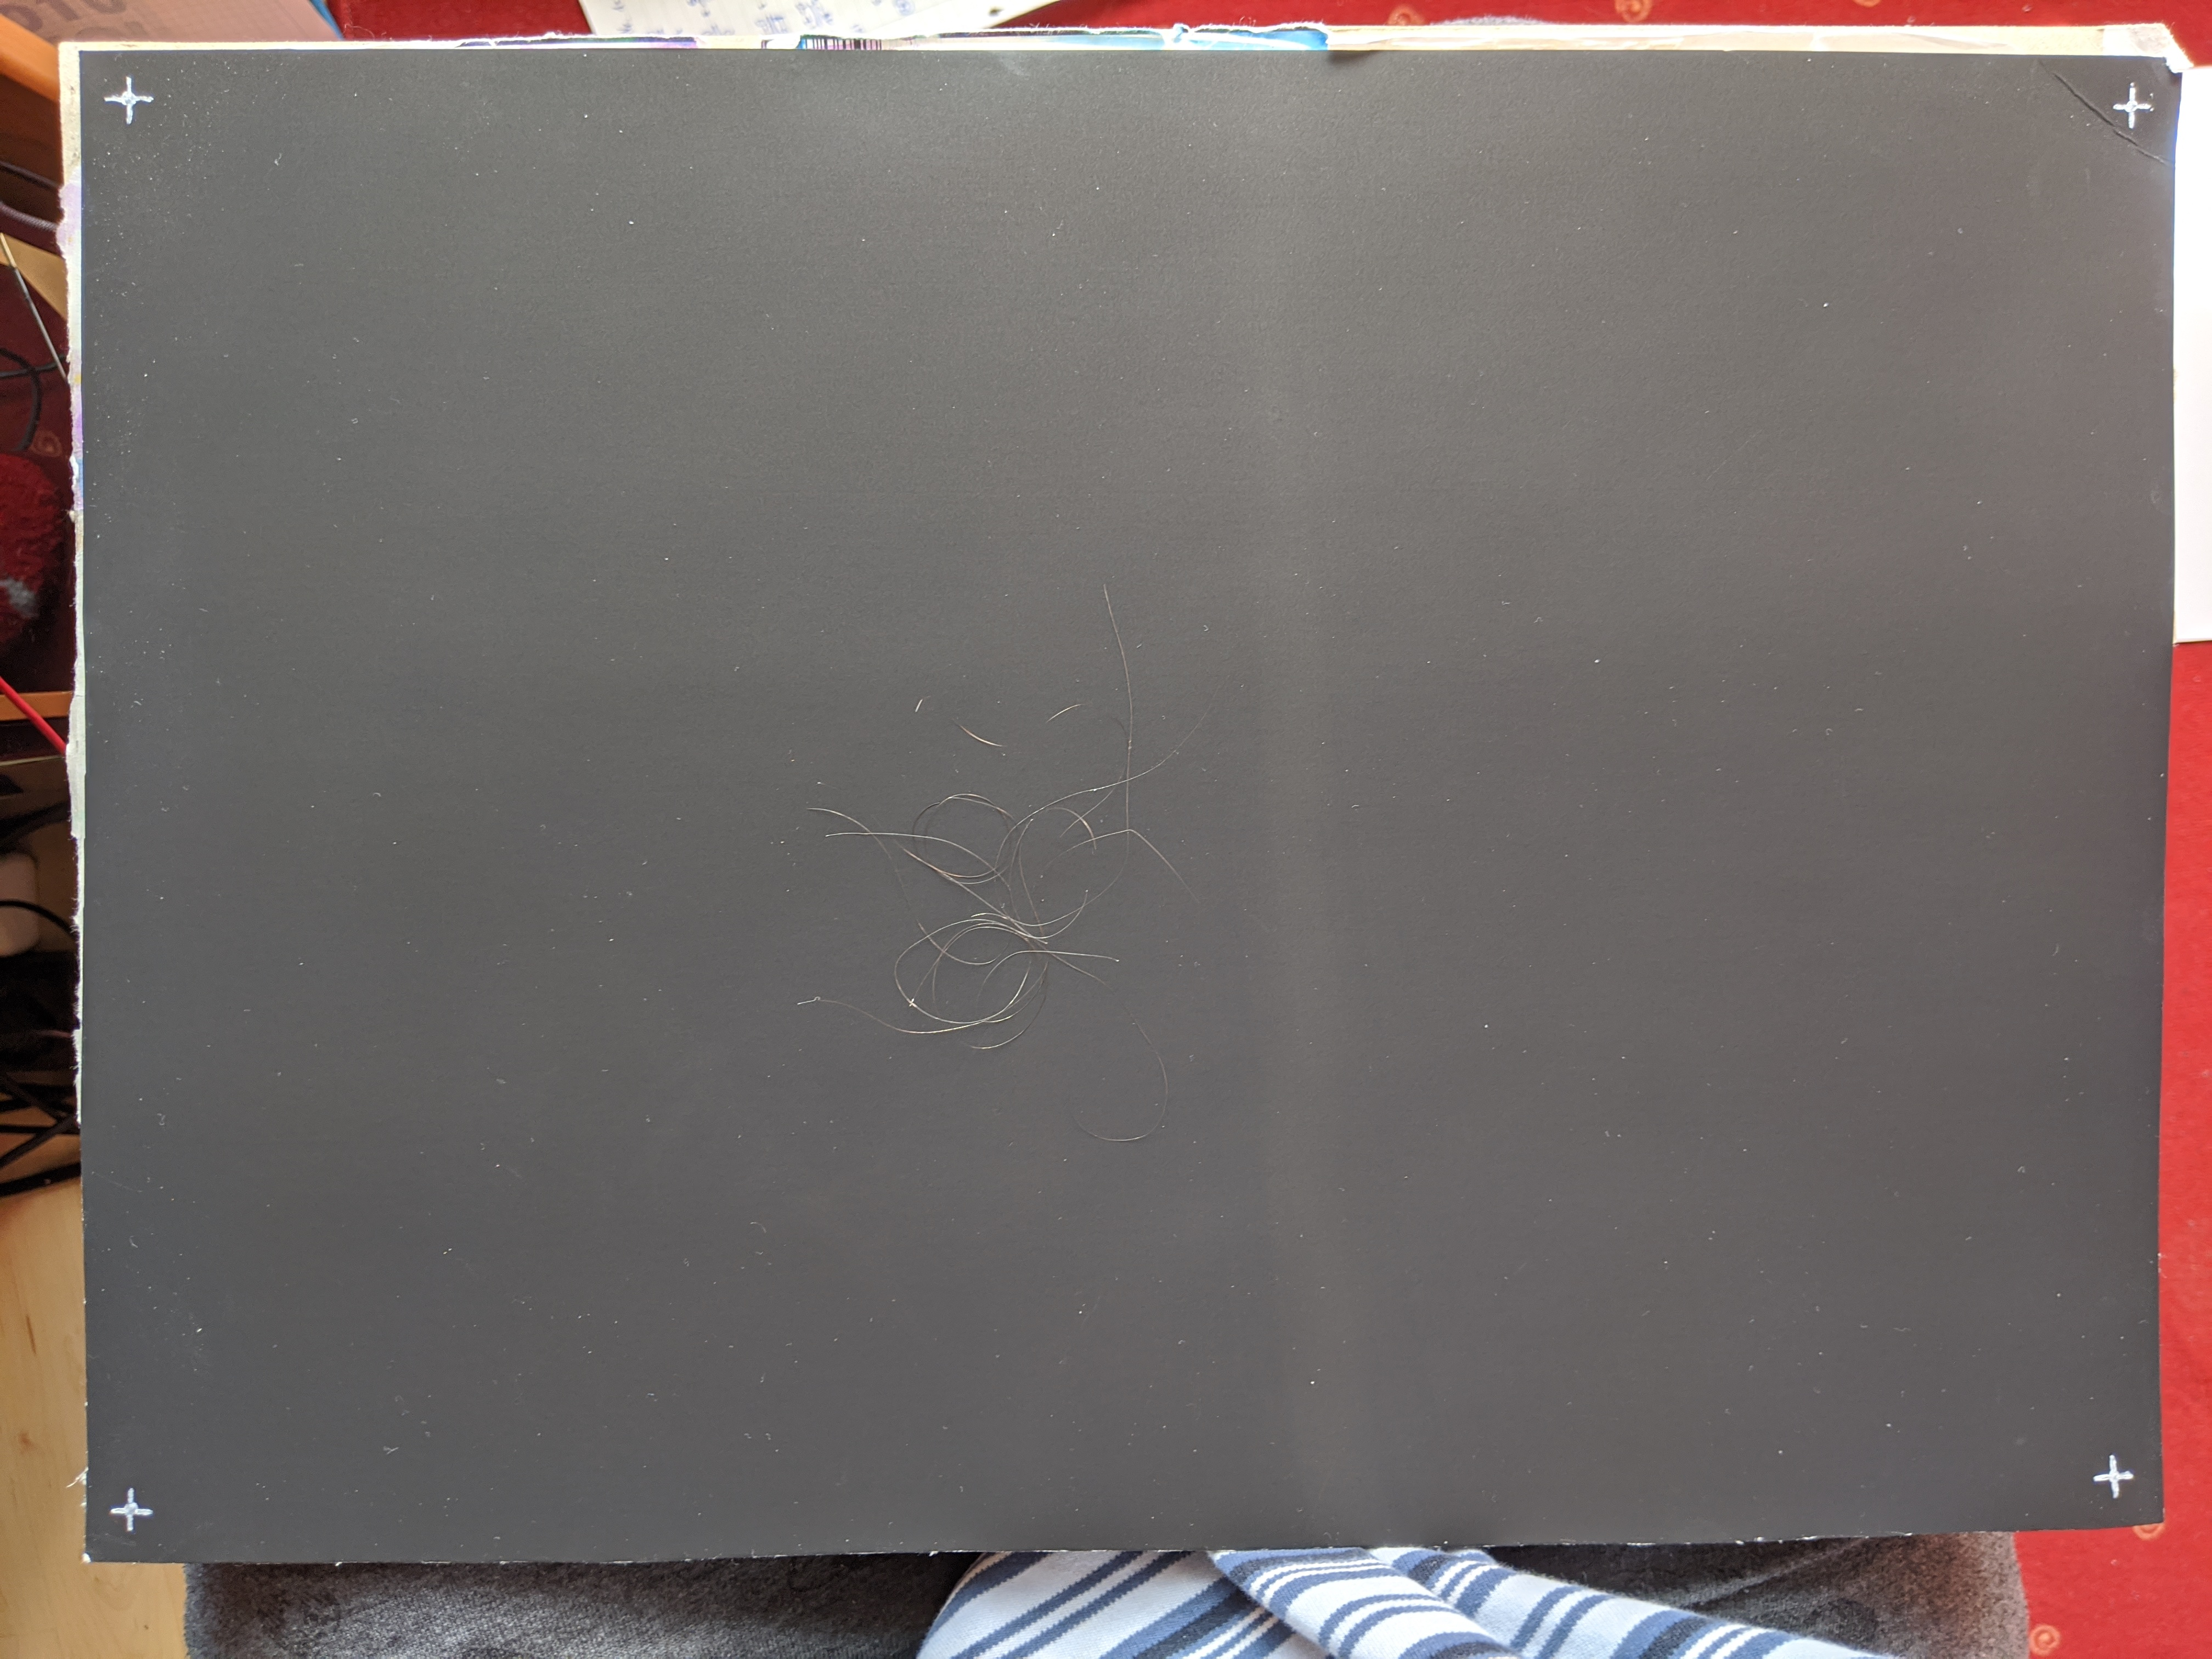
\includegraphics[width=\textwidth]{figJan/IMG_20200325_133957_10.jpg}
		\caption[]{Geschätzt auf 10 Haare. Tatsächlich 10 Haare}
		\label{img:tstJan1} 
	\end{subfigure}
	\hfill
	\begin{subfigure}[b]{0.475\textwidth} 
		\centering
		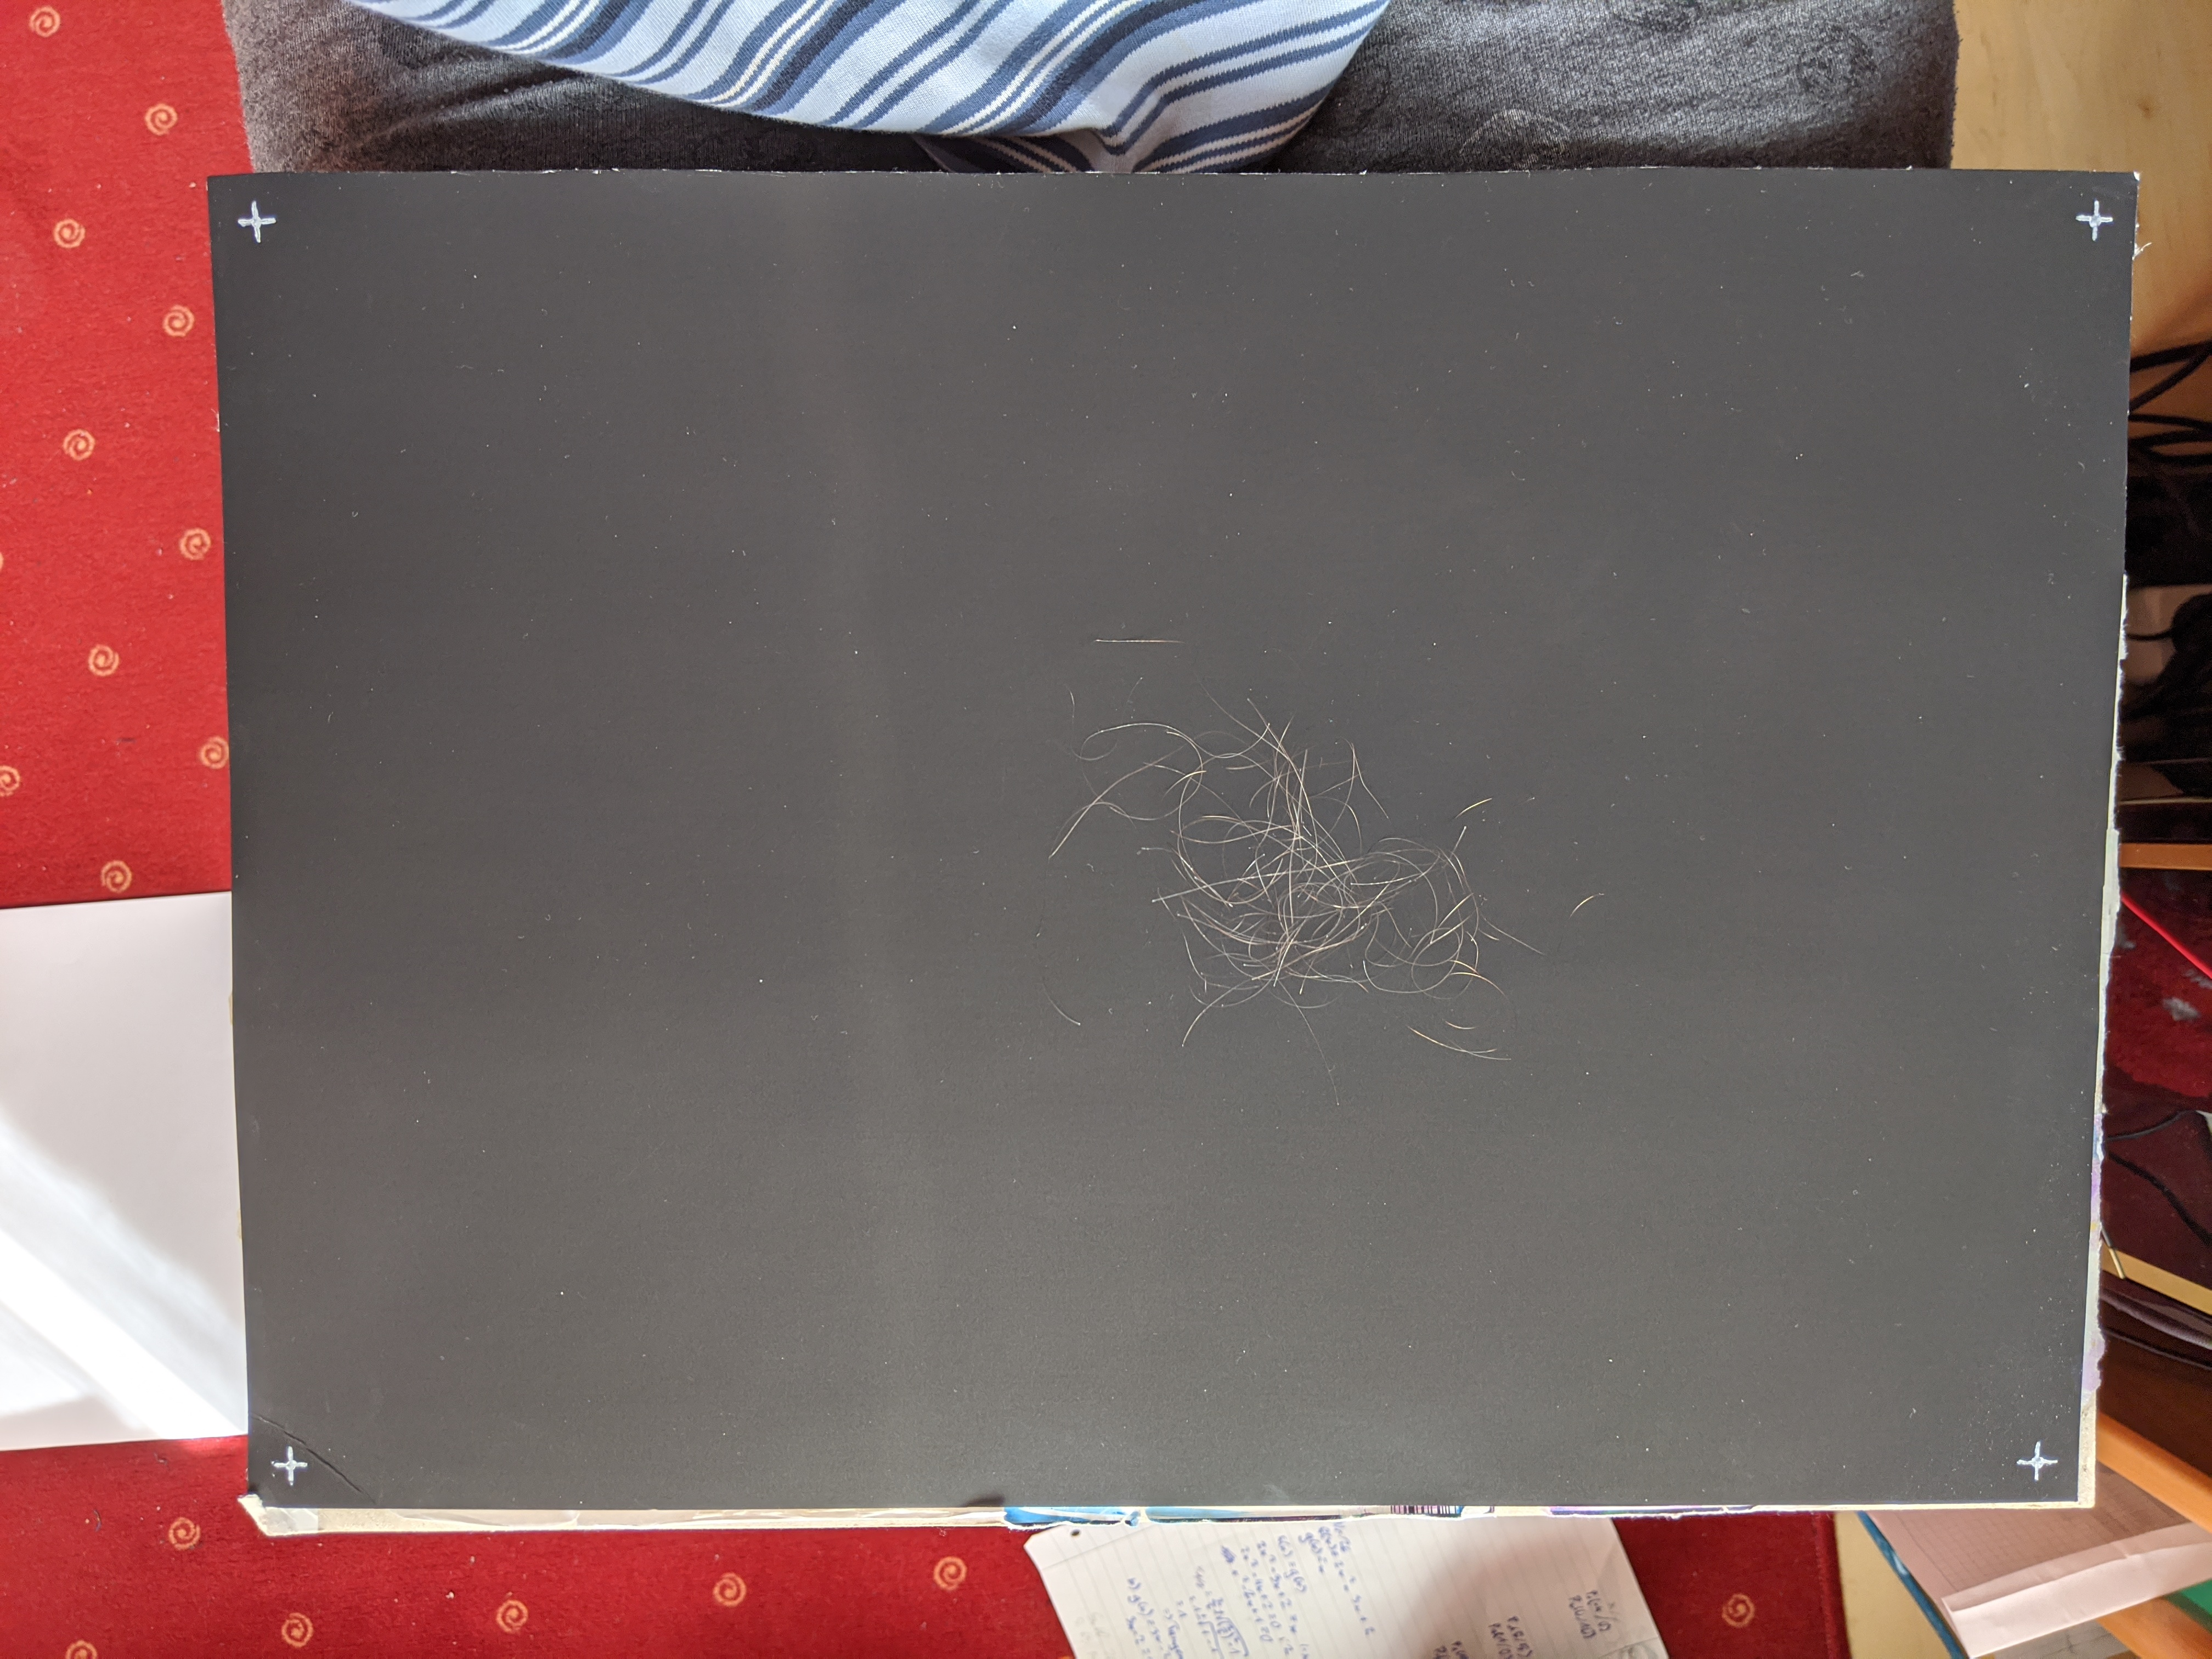
\includegraphics[width=\textwidth]{figJan/IMG_20200325_134303_40.jpg}
		\caption[]{Geschätzt auf 37 Haare. Tatsächlich 40.}
		\label{img:tstJan2}
	\end{subfigure}
	\caption[  ]
	{\small Beispiel input von kurzen Hellbraunen Haaren} 
	\label{img:tstJan}
\end{figure*}

Die Haare sind recht kurz und haben somit weniger Masse, im Vergleich zu den vorherigen Testszenarien. Mit einer Kalibrations-Menge von 3 Bildern ergab sich ein durchschnittlicher Fehler von 2 Haaren über 10 Schätzungen. Der höchste Fehler liegt bei 6, der Niedrigste bei 0.
Siehe Anhang \ref{appendix:Error}.

\subsection{Test: Schulterlange, dunkelbraue Haare}

Dunkele,feine kurze Haare wurden auf weißem Hintergrund aufgenommen. Siehe Abbildung \ref{img:tstMama}

\begin{figure*}
	\centering
	\begin{subfigure}[b]{0.475\textwidth}
		\centering
		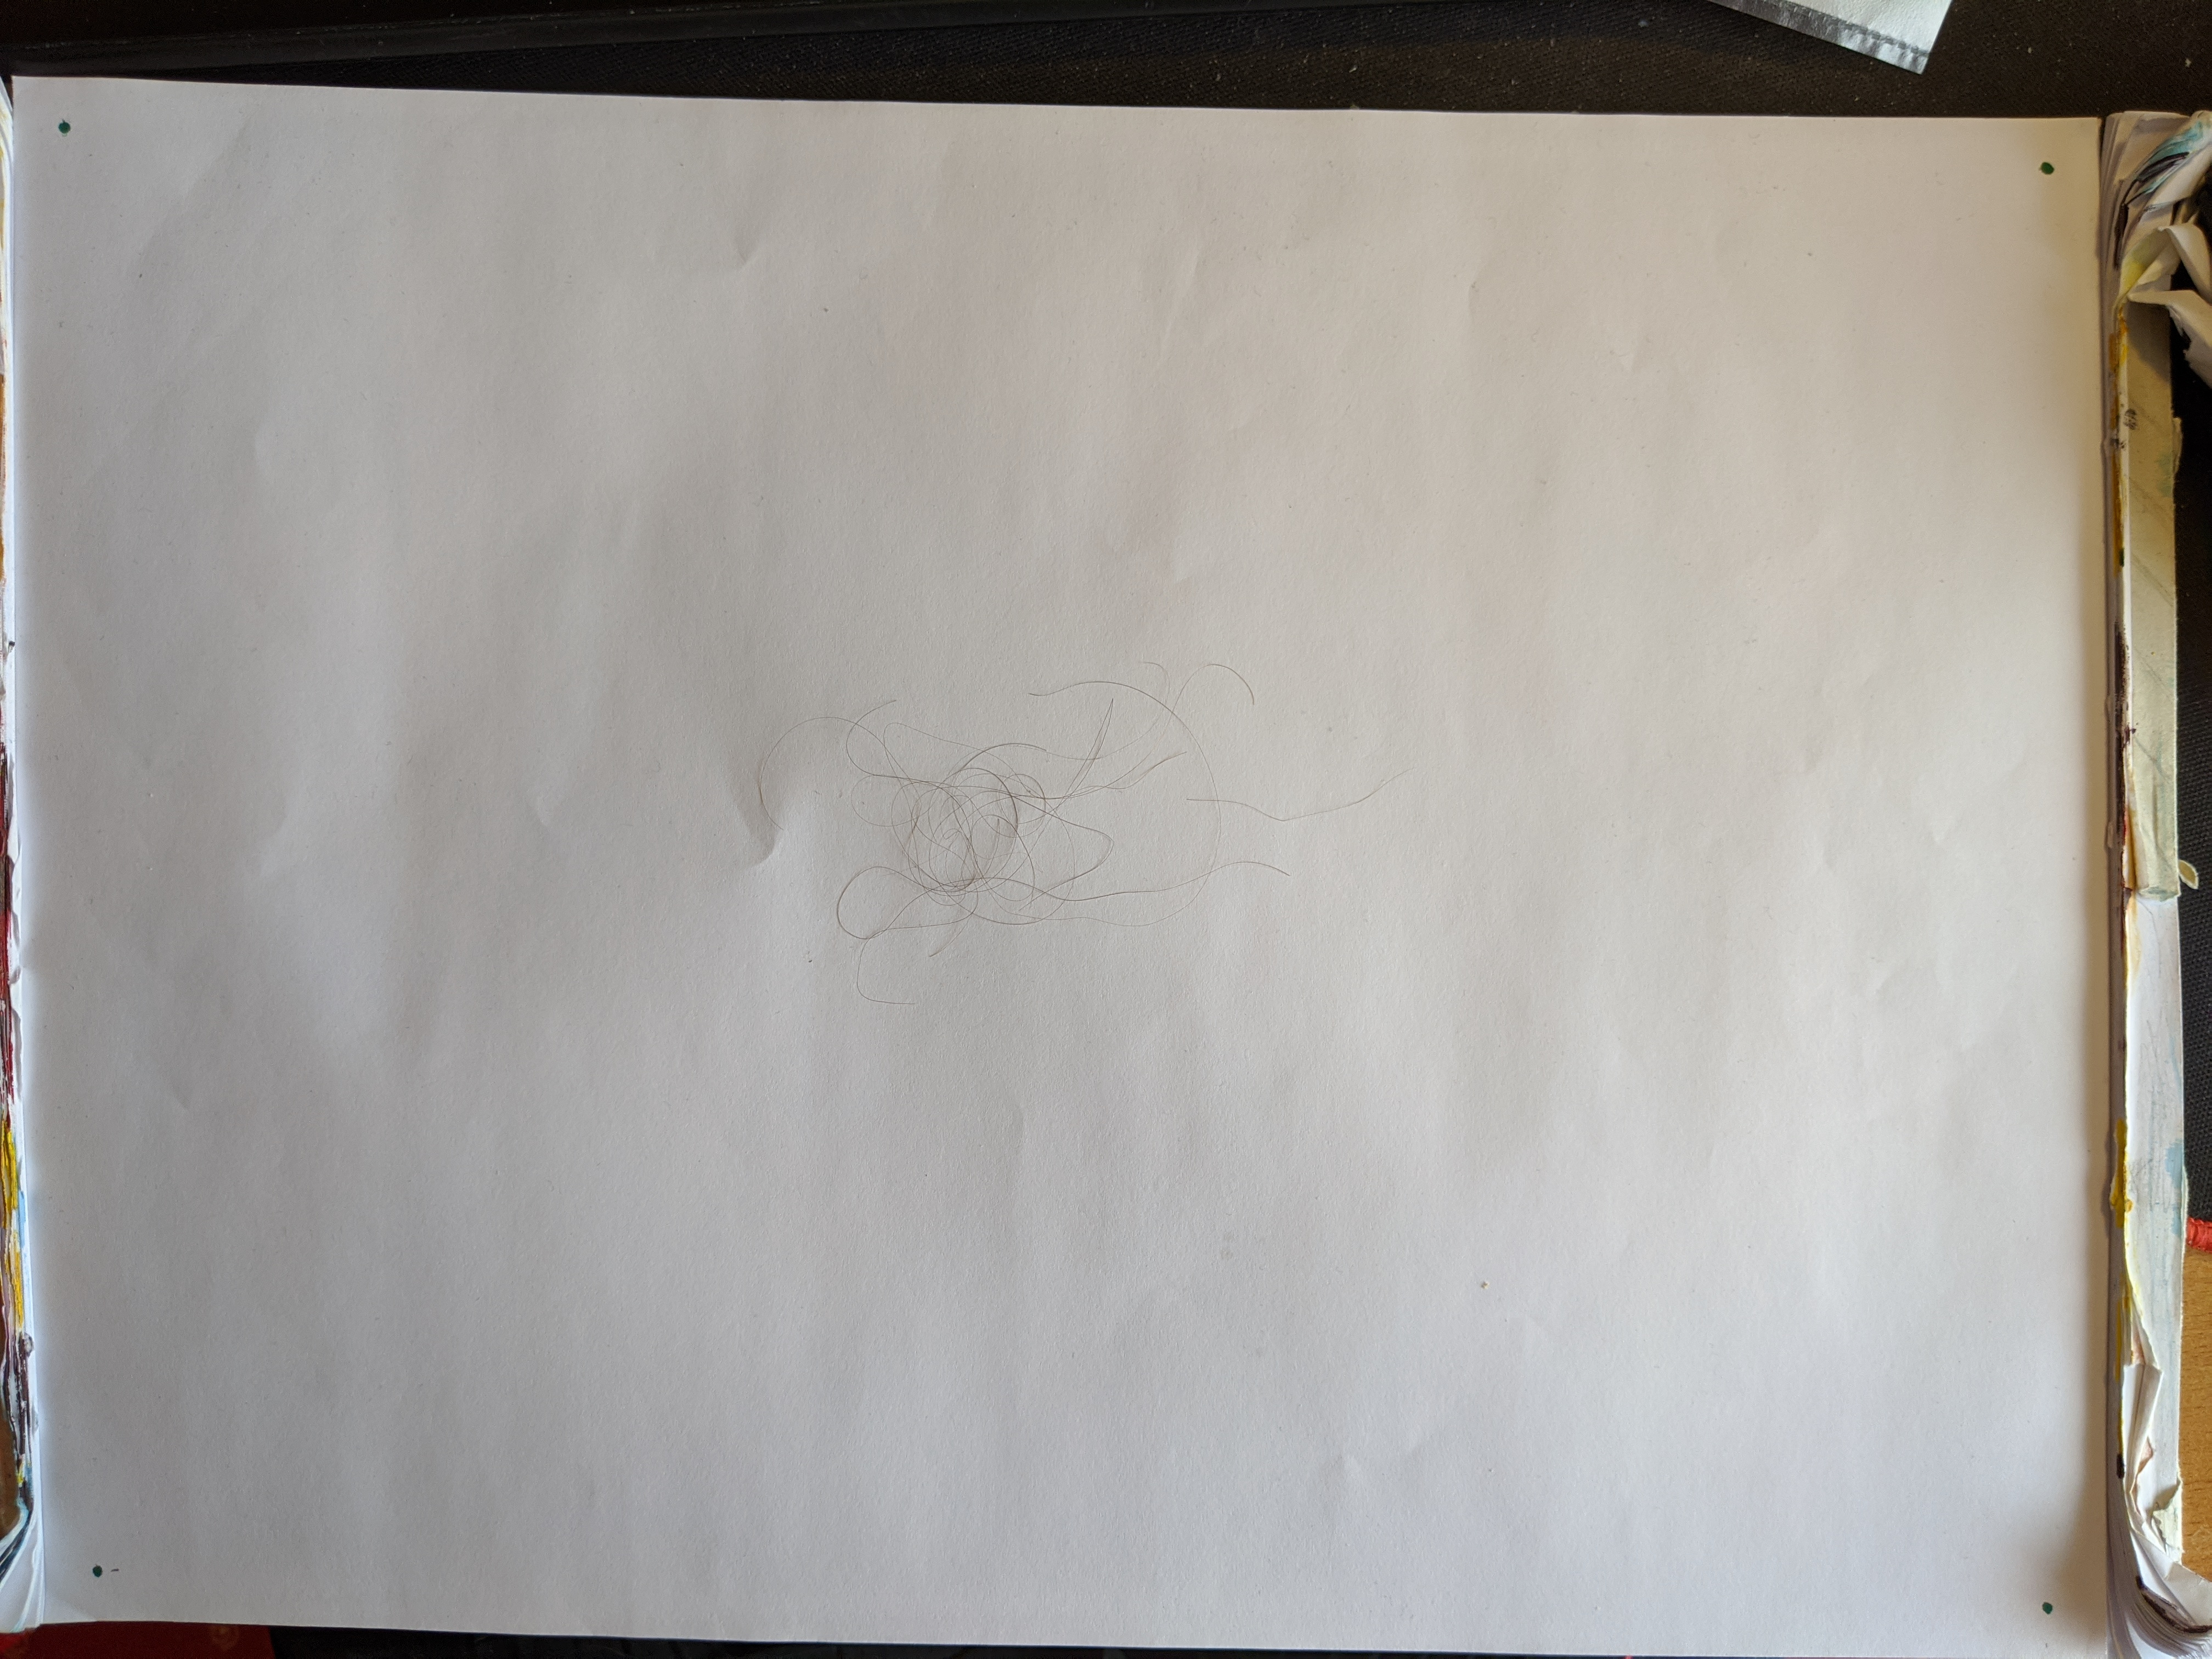
\includegraphics[width=\textwidth]{figMama/IMG_20200327_140450_10.jpg}
		\caption[]{Geschätzt auf 13 Haare. Tatsächlich 10 Haare}
	\end{subfigure}
	\hfill
	\begin{subfigure}[b]{0.475\textwidth} 
		\centering
		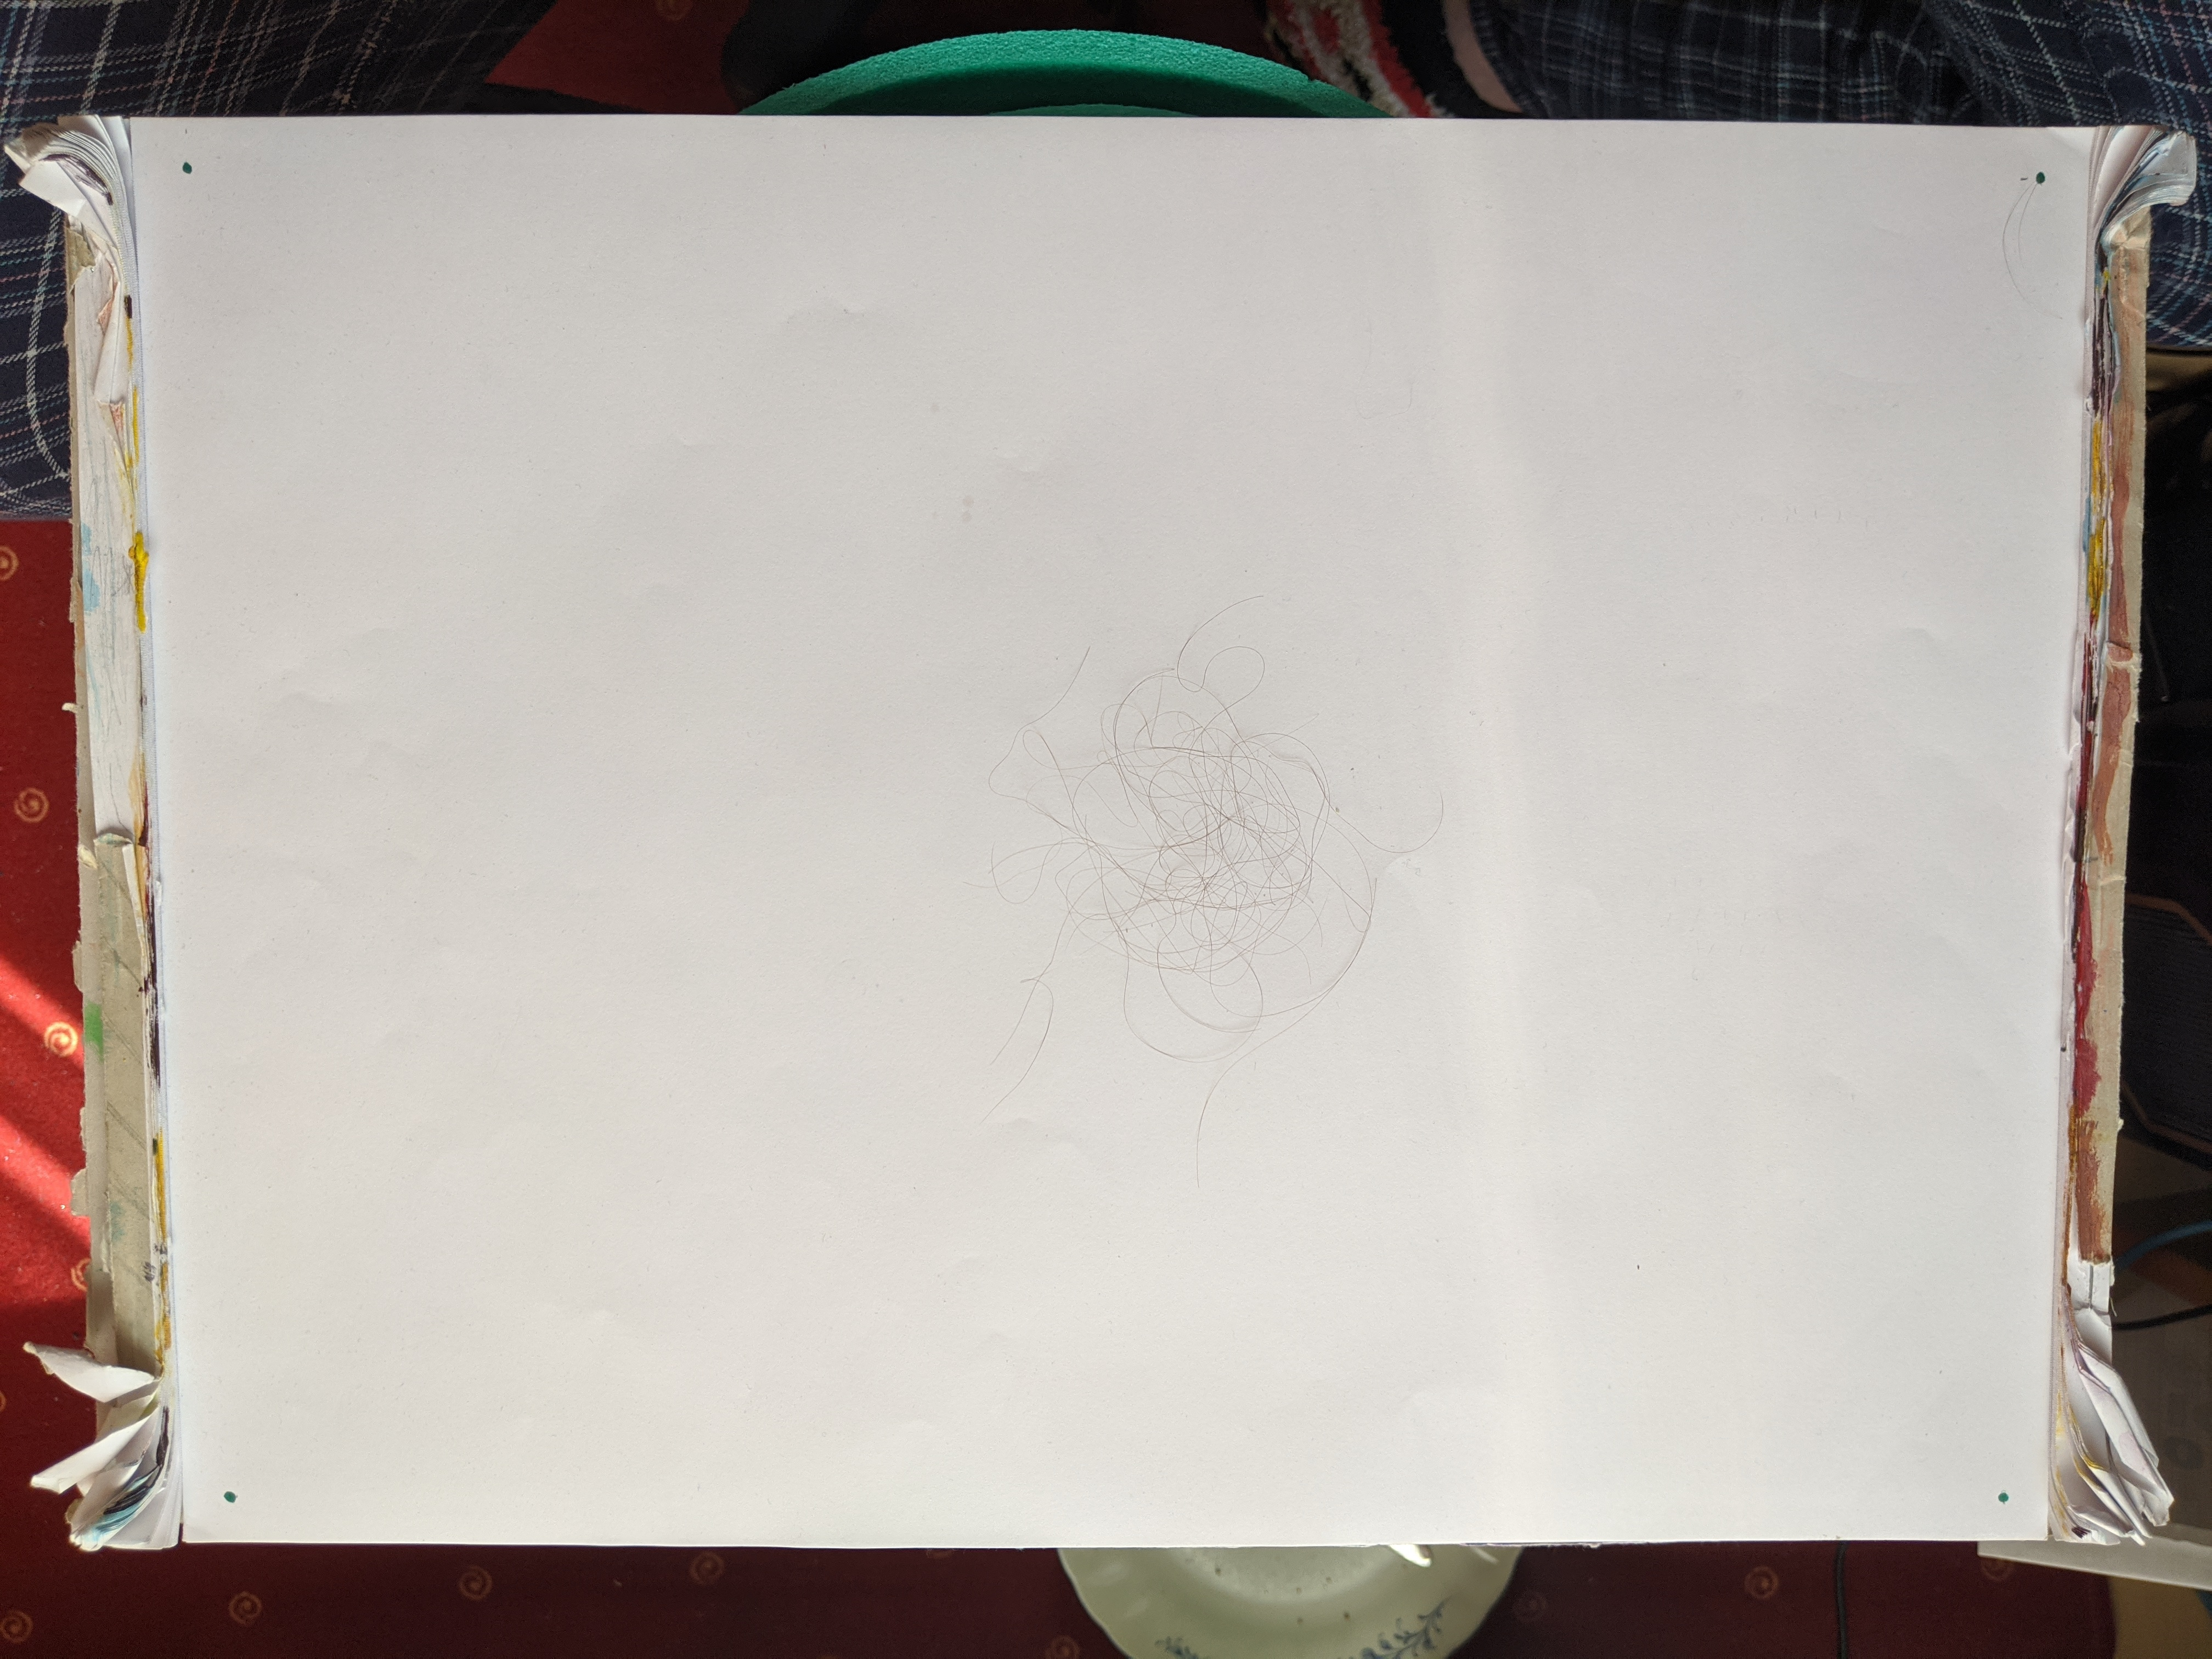
\includegraphics[width=\textwidth]{figMama/IMG_20200330_143938_25.jpg}
		\caption[]{Geschätzt auf 23 Haare. Tatsächlich 25.}
	\end{subfigure}
	\caption[  ]
	{\small Beispiel input von dunkelbraunen Haaren} 
	\label{img:tstMama}
\end{figure*}

Mit 4 Kalibrations-Bildern wurde ein durchschnittlicher Fehler von 1.73 Haaren über 11 Schätzungen gefunden.
Siehe Anhang \ref{appendix:Error}

\section{Ergebnisse}

Durchschnittlich wurden Fehler von 2 bis 5 Haaren pro Schätzung gefunden. In vereinzelten Schätzungen Lag der Fehler bei 16, was ein hoher Fehler ist, wenn nur wenige Haare auf einem Bild zu sehen sind. 
Trotzdem sind die Schätzungen genauer als die Ergebnisse aus dem Paper \blockquote{The Hair shedding visual scale: A quick tool to assess hair loss in Women}. In dem Paper werden Haare in den Inkrementen 10,50,100,200...700 gezählt. \cite{visualScale}

Das Verfahren in dieser Arbeit wurde in dem Bereicht 10 bis 120 Haare getestet und beitet dort eine Höhere Auflösung als Das Paper.\cite{visualScale}

\section{Fazit}
Das Schätzen von der Anzahl an Haaren mithilfe von Bildverarbeitung und statistischer Auswertung zeigt sich als funktionsfähig und effizient. 

In der Zukunft können die unterschiedlichen Schätzungs-Modelle miteinander verglichen werden, um die Kombination der akkuratesten Modelle zu finden. Die Genauigkeit sollte mit noch mehr Haar-Bildern getestet werden. 

Der Bildverarbeitungsprozess braucht recht lange mit 20 bis 30 Sekunden pro Bild. Durch das weglassen von Daten die statistisch nicht ausgewertet werden, sowie das optimieren der Region-Untersuchungen kann der Prozess beschleunigt werden. 

%Es wird eine praktische Methode gegeben eine Langzeitüberwachung von Haarausfall anzustellen. So wird der Anwender sich bewusst, welcher tägliche Haarausfall normal ist und welche Menge besorgniserregend ist. Haarausfall ist sehr variabel und wird durch viele Faktoren beeinflusst. Eine Langzeitüberwachung beruhigt den Nutzer bei saisonalem Haarausfall und gibt Hinweise auf die allgemeine Gesundheit der Haare. Die Langzeitüberwachung macht den Haarausfall transparenter und berechenbarer. So wird der Nutzer früher aufmerksam auf anomalen Haarausfall und kann darauf besser reagieren.

\newpage

\nocite{*}
\printbibliography

\appendix
\section{28 Datenpunkte pro Bild}
\label{appendix:datenpunkte}

\begin{itemize}
	\item intensitySum - Summe der Graustufenwerte des Intensität-Bildes
	\item intensityShare - Intensität pro HaarPixel
	\item hairpixels - Anzahl der Pixel, die Haare darstellen
	\item imagepixels - Gesammtanzahl der Pixel im Bild
	\item hairpixel percentage - Prozentsatz der Haarpixel im Bild
	\item number of sections - Anzahl an Hintergrund Regionen, die Watershed findet.
	\item number of background sections - Anzahl an Regionen, die den Hintergrund darstelle. (2 weniger als number of section. Watershed zählt Haare und übergänge zwischen Regionen mit)
	\item outerSectionSum - Summe an Pixeln, die sich in der Region befinden, die die Haare umschließt
	\item outerSectionPercentage - outerSectionSum/imagepixels
	\item innerSectionSum - Summa an Pixeln, die sich in Regionen befinden, die von Haaren umschlossen werden
	\item innserSectionAvgSize - Druchschnittliche Pixelanzahl, die sich in den umschlossenen Regionen befinden
	\item innerSectionAvgSize Percentage - innersectionAvgSize/imagepixels
	\item innerSectionSizeVariance - statistische Varianz der Pixelmengen, die sich in umschlossenen Regionen befinden
	\item innerSection standard deviation - Standardabweichung der Pixelmengen, die sich in umschlossenen Regionen befinden
	\item number of sections only concidering dense hair - Anzahl der Regionen, die Watershed findet nachdem der input Skelettiert wurde. Regionen werden von dichteren Haaren unterteilt.
	\item number of background sections inclosed by dense hair - Anzahl an Regionen, die den Hintergrund zwischen dichten Haaren darstellen
	\item dense hair outerSectionSum - Summe an Pixeln, die die Regionen umschließen, die von dichten Haaren umschlossen werden
	\item dense outerSectionPercentage - dense hair outerSectionSum / imagepixels
	\item dense innerSectionSum - Summe an Pixeln, die sich in den Regionen befinden, die von dichten Haaren umschlossen werden
	\item dense hair innserSectionAvgSize - Durschnittliche anzahl der Pixel, die sich in Regionen befinden, die von dichten Haaren umschlossen werden
	\item dense hair innerSectionAvgSize Percentage - dense hair innerSectionAvgSize / imagepixels
	\item dense innerSectionSizeVariance - statistische Varianz in den Größen der Regionen, die von dichten Haaren umschlossen werden
	\item dense innerSection Size standard deviation - Standardabweichung der Pixelmengen
	\item denseHairSum - Summe an Pixeln, die als Dichte Haare angesehen werden
	\item looseHairSum - Summe an Pixeln, die als Haare angesehen werden, jedoch nicht als Dicht gelten
	\item IntensitySum in Loose Section - Summe der Graustufenwerte in nicht-dichten Regionen
	\item IntensitySum in Dense Section - Summe der Graustufenwerte in dichten Regionen
\end{itemize}

\section{x Wert Berechnungen für Schätzungs-Modelle}
\label{appendix:xwertemodel}
\begin{itemize}
	\item hairpercent 
	\begin{itemize}
		\item Prozentsatz der Haarpixel im Bild.
	\end{itemize}
	\item (hairpixels / hairSectionSize) * (1 - outerSectionPerc)
	\begin{itemize}
		\item HaarPixel Dichte in der Region, in der sich Haare befinden. Gibt dasselbe Ergebnis wie hairpercent.
	\end{itemize}
	\item (hairpixels/hairSectionSize)*(1-outerSectionPerc)*hairPerc
	\item (((denseHairSum / denseInnerSectionSize) * (1 - denseSectionperc))) = denseDensity
	\begin{itemize}
		\item Dichte in den Dichten Regionen.
	\end{itemize}
	\item denseDensity / looseDensity
	\begin{itemize}
		\item Verhältnis dichte Regionen zu loosen Regionen.
	\end{itemize}
	\item backgroundSectionNum*(1-outerSectionPerc)
		\begin{itemize}
		\item Anzahl der HintergrundRegionen in Region, in der sich Haare Befinden.
	\end{itemize}
	\item denseSectionNum*(1-outerSectionPerc)
		\begin{itemize}
		\item Anzahl der HintergrundRegionen, die von dichten Haaren getrennt sind, in Haar-Region.
	\end{itemize}
	\item intensitySum*hairpixels*(1-outerSectionPerc)
	\begin{itemize}
		\item Intensitäts Summe pro HaarPixel in Haar-Region.
	\end{itemize}
	\item denseSectionAVGSize/(1-denseSectionperc)
		\begin{itemize}
		\item Durchschnittliche Größe der HintergrundRegionen, die durch dichte Haare getrennt sind.
	\end{itemize}
	\item (denseSectionAVGSize/looseSectionAVGSize)/(1-outerSectionPerc)
		\begin{itemize}
		\item Durchschnittliche Größe von Hintergrundregionen in dichten Regionen verglichen mit Durchschnittlicher Größe von Hintergrundregionen in loosen Regionen.
	\end{itemize}
	\item (denseIntensity/intensitySum)*(1-denseSectionperc)
		\begin{itemize}
		\item Intensität in Dichten Regionen verglichen mit gesammter Intensität.
	\end{itemize}
	\item (denseIntensity/denseHairSum)*(1-denseSectionperc)
		\begin{itemize}
		\item Intensität in Dichten Regionen verglichen mit Summe an Haarpixeln, die als dicht gelten.
	\end{itemize}
\end{itemize}

\newpage

\section{Schätzungs Modelle}
\label{appendix:modelle}
\begin{figure}[H] % "[t!]" placement specifier just for this example
\begin{subfigure}{0.48\textwidth}
	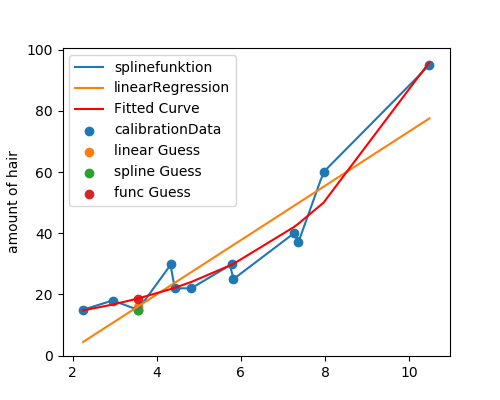
\includegraphics[width=1.1\linewidth]{fig64/g01_hairpercent.png}
	\caption{hairpercent} \label{fig:a}
\end{subfigure}\hspace*{\fill}
\begin{subfigure}{0.48\textwidth}
	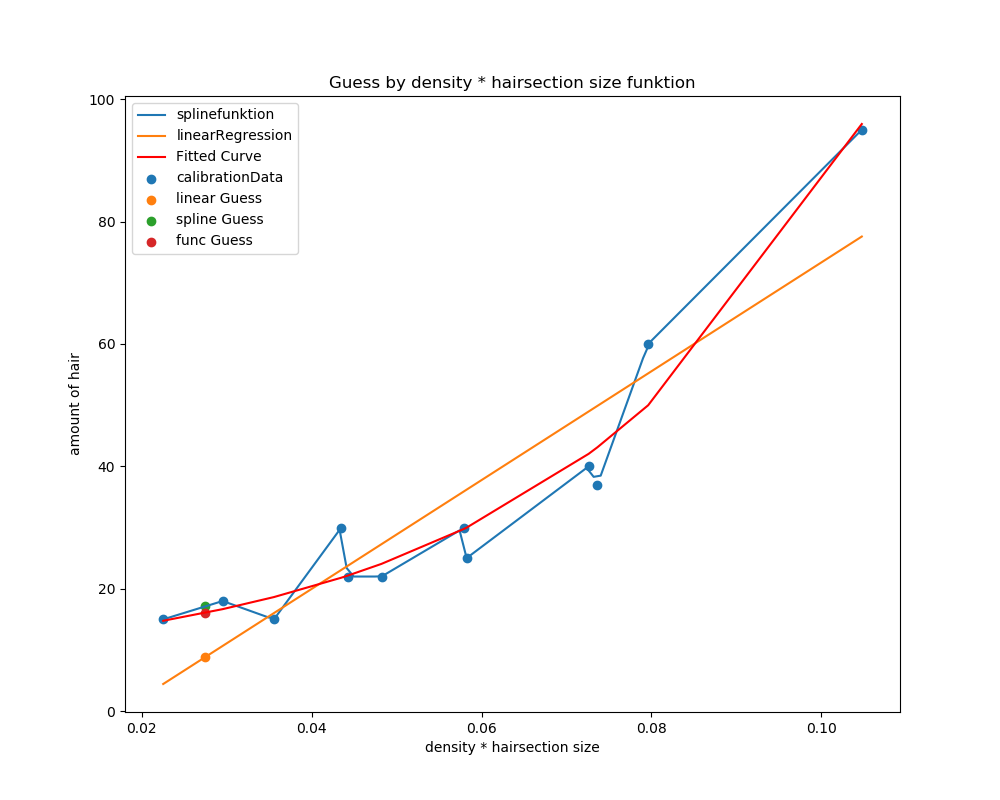
\includegraphics[width=1.1\linewidth]{fig64/g02_densitynorm.png}
	\caption{density*hairsection size} \label{fig:b}
\end{subfigure}

\medskip
\begin{subfigure}{0.48\textwidth}
	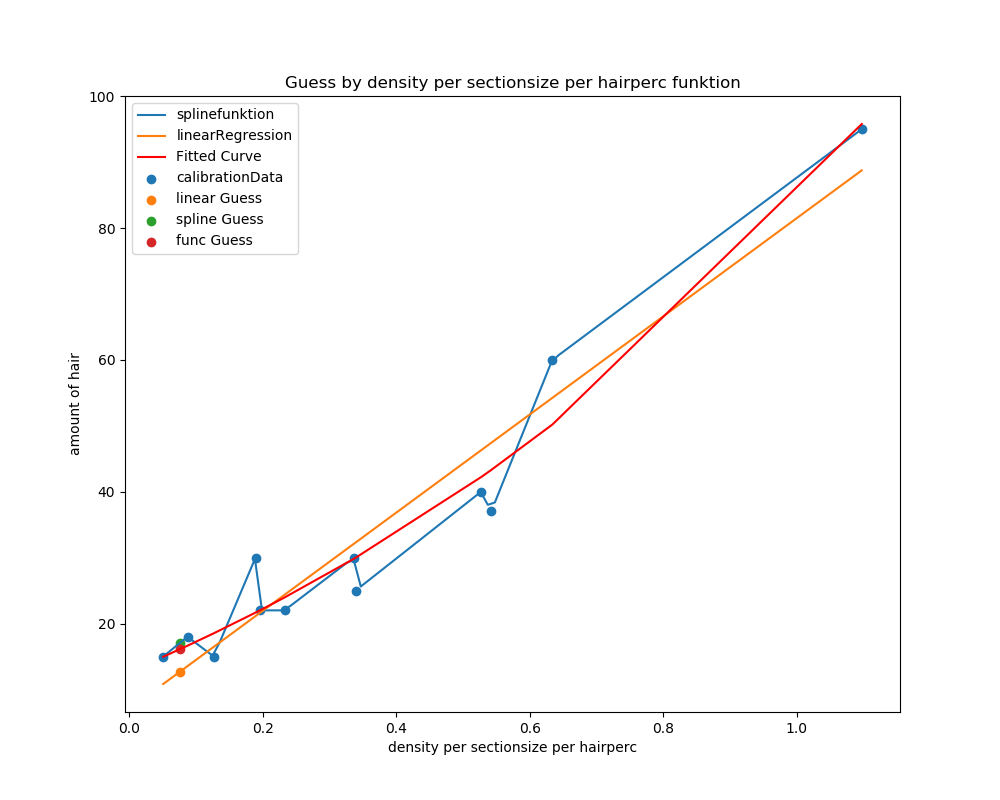
\includegraphics[width=1.1\linewidth]{fig64/g03_densitynorm2.png}
	\caption{density per sectionsize per hairperc} \label{fig:c}
\end{subfigure}\hspace*{\fill}
\begin{subfigure}{0.48\textwidth}
	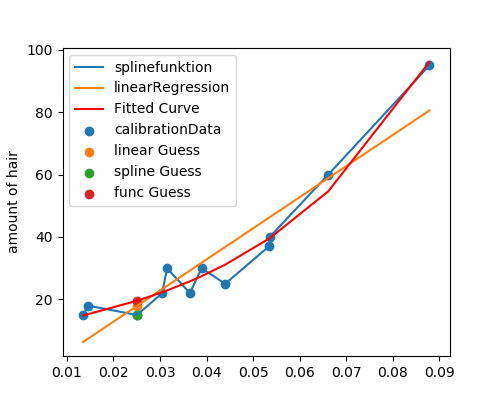
\includegraphics[width=1.1\linewidth]{fig64/g04_densityDenseSections.png}
	\caption{density of dense section in relation to section size} \label{fig:d}
\end{subfigure}

\medskip
\begin{subfigure}{0.48\textwidth}
	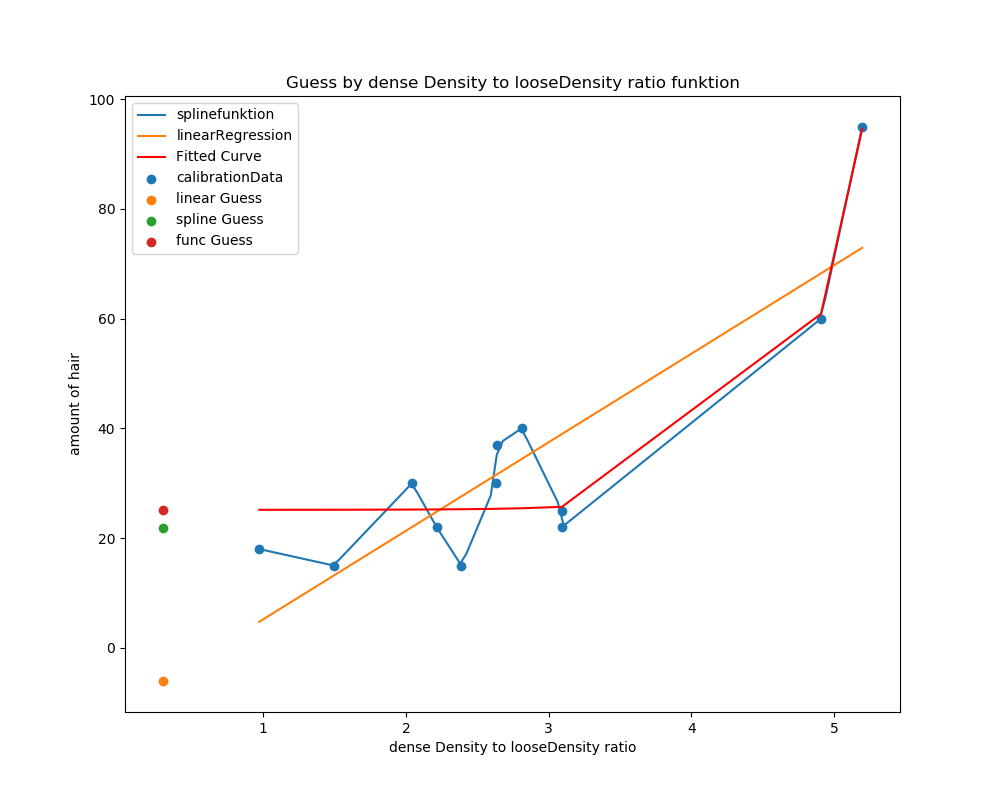
\includegraphics[width=1.1\linewidth]{fig64/g05_denseDensitytolooseDensity.png}
	\caption{dense Density to loose Density ratio} \label{fig:e}
\end{subfigure}\hspace*{\fill}
\begin{subfigure}{0.48\textwidth}
	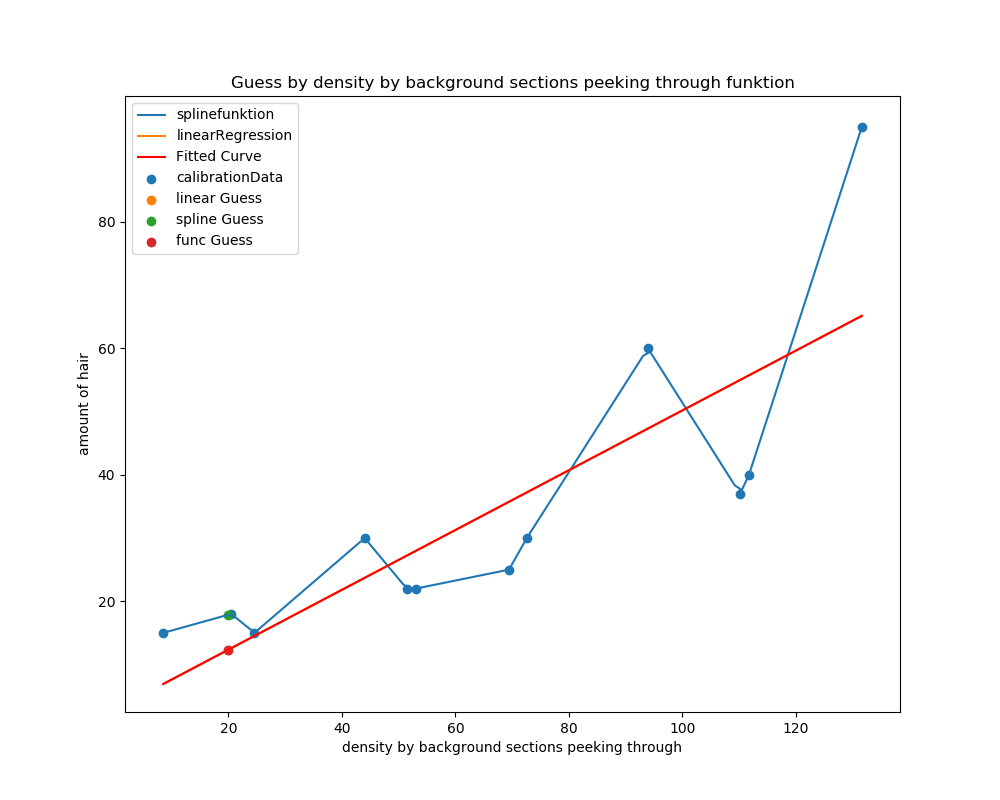
\includegraphics[width=1.1\linewidth]{fig64/g06_densitybybackgorundsections.png}
	\caption{density by background section peeking through} \label{fig:f}
\end{subfigure}


\caption{Schätzungsmodelle angewandt auf lange rotbraune Haare (1)} \label{fig:1}
\end{figure}

\begin{figure}[H] % "[t!]" placement specifier just for this example
	\begin{subfigure}{0.48\textwidth}
		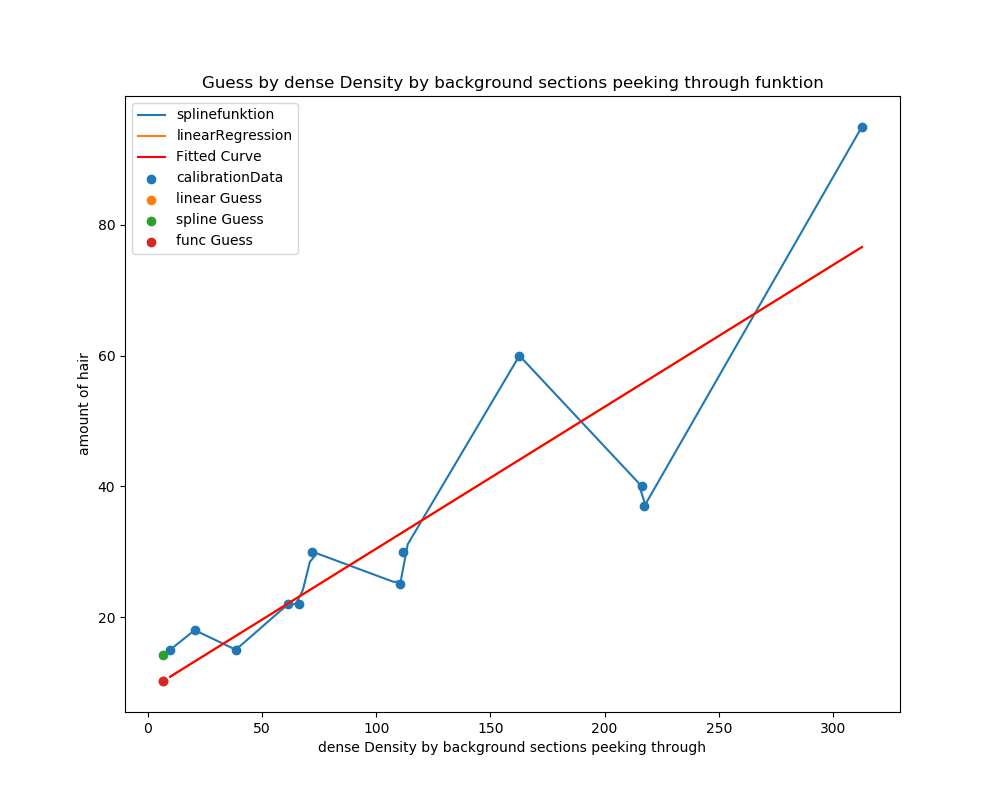
\includegraphics[width=1.15\linewidth]{fig64/g07_denseDensitybyBackgroundSections.png}
		\caption{dense Density by background section peeking through} \label{fig:a}
	\end{subfigure}\hspace*{\fill}
	\begin{subfigure}{0.48\textwidth}
		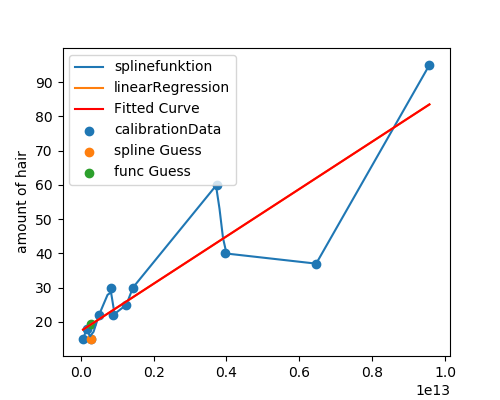
\includegraphics[width=1.15\linewidth]{fig64/g08_intensitynorm.png}
		\caption{intensity in relation to hairPixels and hairsectionsize} \label{fig:b}
	\end{subfigure}
	
	\medskip
	\begin{subfigure}{0.48\textwidth}
		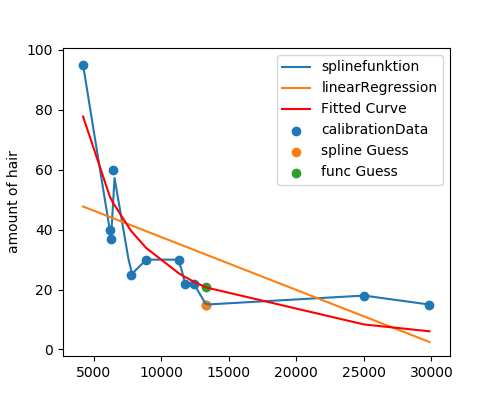
\includegraphics[width=1.15\linewidth]{fig64/g09_avgbackgroundsectionsizes.png}
		\caption{average background section sizes in dense section} \label{fig:c}
	\end{subfigure}\hspace*{\fill}
	\begin{subfigure}{0.48\textwidth}
		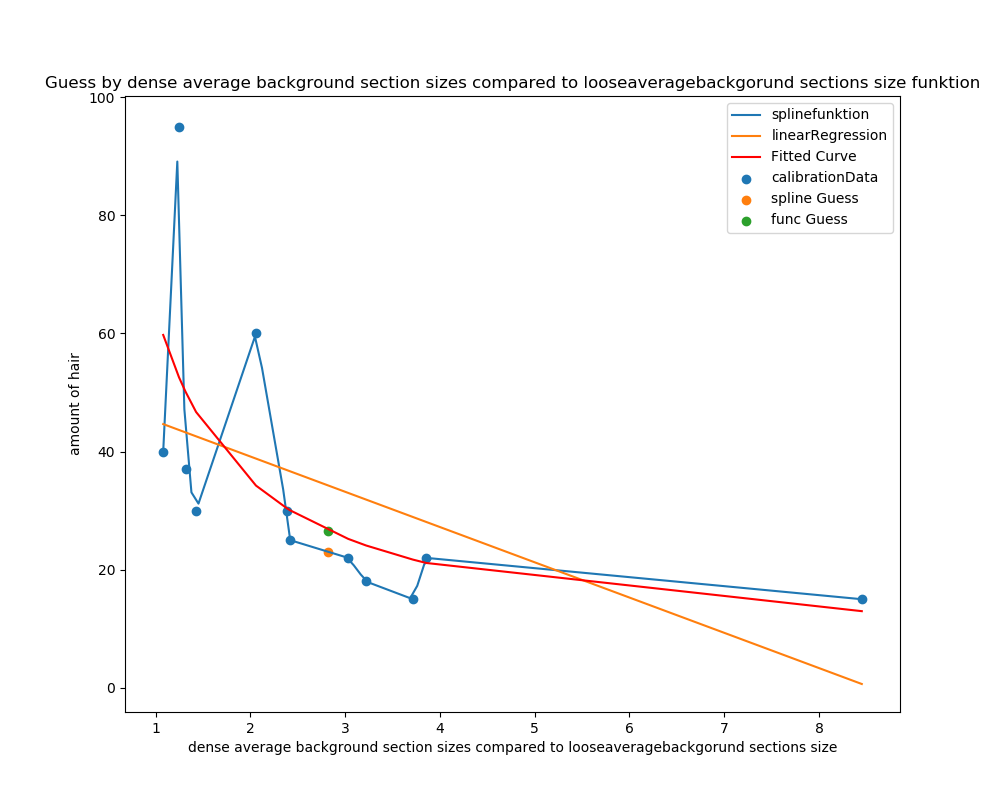
\includegraphics[width=1.15\linewidth]{fig64/g10_denseavgbackgroundsizeVSlooseavg.png}
		\caption{dense average background section size compared to looseaveragebackground section size} \label{fig:d}
	\end{subfigure}
	
	\medskip
	\begin{subfigure}{0.48\textwidth}
		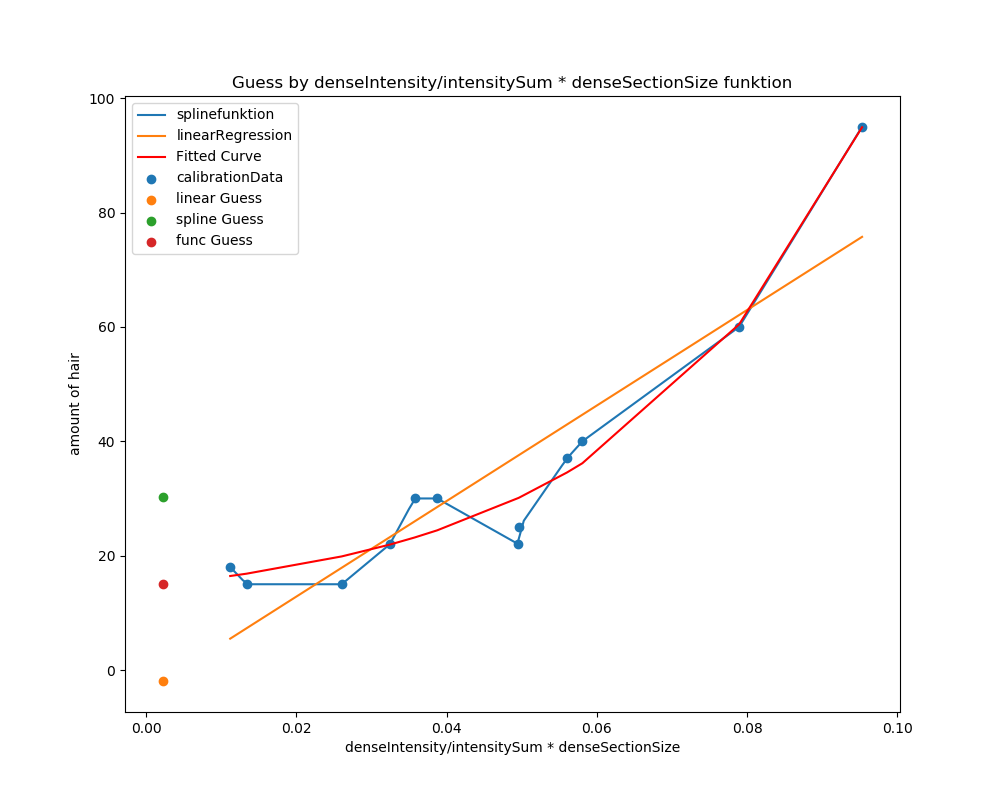
\includegraphics[width=1.15\linewidth]{fig64/g11_denseIntensitynorm.png}
		\caption{densityIntensity/intensitySum * denseSectionSize} \label{fig:e}
	\end{subfigure}\hspace*{\fill}
	\begin{subfigure}{0.48\textwidth}
		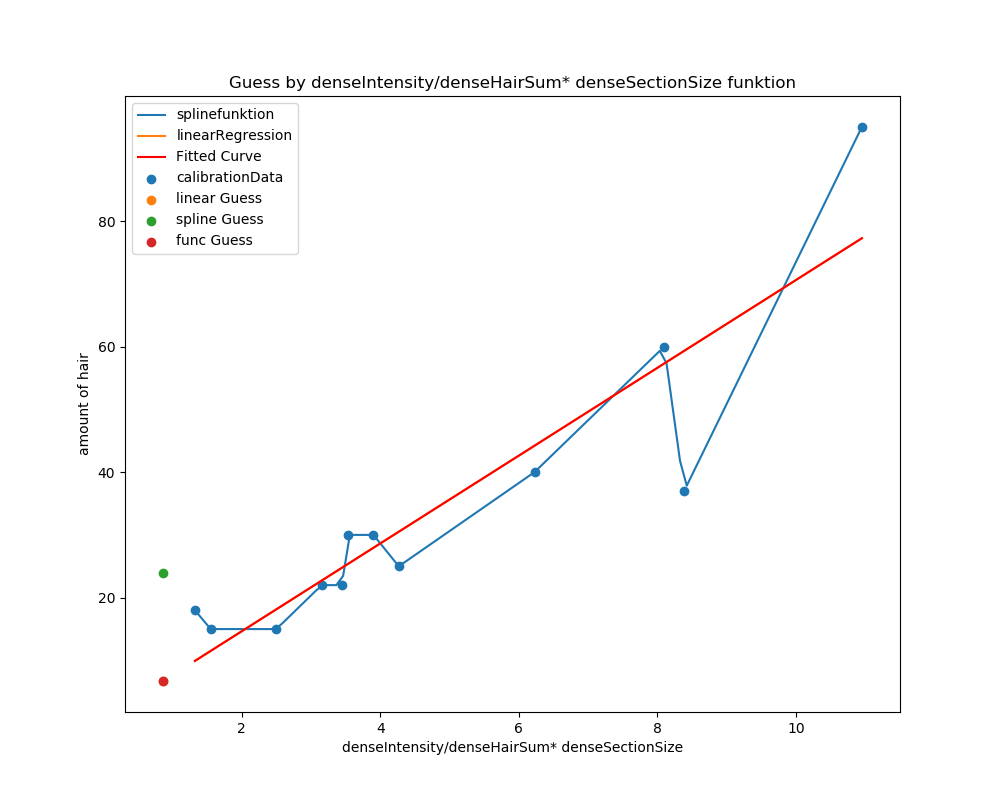
\includegraphics[width=1.15\linewidth]{fig64/g12_denseIntensitynorm2.png}
		\caption{denseIntensity/denseHairSum * denseSectionSize} \label{fig:f}
	\end{subfigure}
	
	
	\caption{Schätzngsmodelle angewandt auf lenge rotbraune Haare (2)} \label{fig:1}
\end{figure}


\section{Kommandozeilen Aufruf einer Schätzung}
\label{appendix:komm}

\begin{lstlisting}[style=DOS]
D:\Eigene Dateien\Dokumente\GitHub\HairEstimation
\HairEstimationPython>python Estimation.py 
guess Users/Mummel/estimationInput/IMG_20200421_170027.jpg -t
active user: Mummel

guessing the amount of hair in the picture
started processing at 2020-04-24 16:16:17.439259
image path Users/Mummel/estimationInput/
IMG_20200421_170027.jpg
cropping image to TemplateDot using PatternMatching
Users/Mummel
2020-04-24 16:16:18.276991 elapsed time 0:00:00.837732
2020-04-24 16:16:18.278993 elapsed time 0:00:00.002002
detecting Hair via edge detection
2020-04-24 16:16:18.296987 elapsed time 0:00:00.017994
backgroundcolor 138.58104800277272
removing smaller Regions...
done
2020-04-24 16:16:19.594080 elapsed time 0:00:01.297093
2020-04-24 16:16:19.602077 elapsed time 0:00:00.007997
processing background regions...
innerSectionNum 434
looping though sections took: 0:00:07.039282
done
2020-04-24 16:16:26.883283 elapsed time 0:00:07.281206
skeletonize
skeletonizing took 0:00:00.279913
processing background regions...
innerSectionNum 578
looping though sections took: 0:00:09.473014
done
2020-04-24 16:16:36.888129 elapsed time 0:00:10.004846
2020-04-24 16:16:36.983098 elapsed time 0:00:00.094969
Image Processing took : 0:00:19.543839
Guess by hairpercent 
[ spl 30.04 ;func 33.50 ;linguess 40.48 ]
Guess by density * hairsection size 
[ spl 30.04 ;func 33.50 ;linguess 40.48 ]
Guess by density per sectionsize per hairperc 
[ spl 29.68 ;func 33.57 ;linguess 36.66 ]
Guess by density of dense section in 
realtion to section size 
[ spl 27.13 ;func 23.87 ;linguess 26.09 ]
Guess by dense Density to looseDensity ratio 
[ spl 17.17 ;func 25.16 ;linguess 7.08 ]
Guess by density by background sections peeking through 
[ spl 23.50 ;func 31.84 ;linguess 31.84 ]
Guess by dense Density by background sections peeking through 
[ spl 28.77 ;func 26.45 ;linguess 26.45 ]
Guess by intensity in relation to hairPixels 
and hairsection size 
[ spl 41.49 ;func 44.53 ]
Guess by average backgorund section sizes in dense section 
[ spl 22.00 ;func 22.97 ]
Guess by dense average background section sizes 
compared to looseaveragebackgorund sections size
[ spl 34.09 ;func 44.39 ]
Guess by denseIntensity/intensitySum * denseSectionSize 
[ spl 15.00 ;func 18.82 ;linguess 14.69 ]
Guess by denseIntensity/denseHairSum* denseSectionSize 
[ spl 37.29 ;func 41.73 ;linguess 41.73 ]
[40.48 30.04 33.50 40.48 30.04 33.50 36.66 
29.68 33.57 26.09 27.13 23.87 7.08 17.17 25.16
31.84 23.50 31.84 26.45 28.77 26.45 41.49 44.53 22.00
22.97 34.09 44.39 14.69 15.00 18.82 41.73 37.29 41.73]
outliers Removed [30.04 33.50 30.04 33.50 36.66 29.68
33.57 26.09 27.13 23.87 25.16 31.84 23.50 31.84 26.45 
28.77 26.45 22.00 22.97 34.09 37.29]
mean 29.258996555560998 res 29.0
saving data point 2020-04-21 29.0 
ImagePath: 
Users/Mummel/estimationInput/IMG_20200421_170027.jpg
\end{lstlisting}

\section{Blondes Haar}

\begin{figure}[H] % "[t!]" placement specifier just for this example
	\begin{subfigure}{0.48\textwidth}
		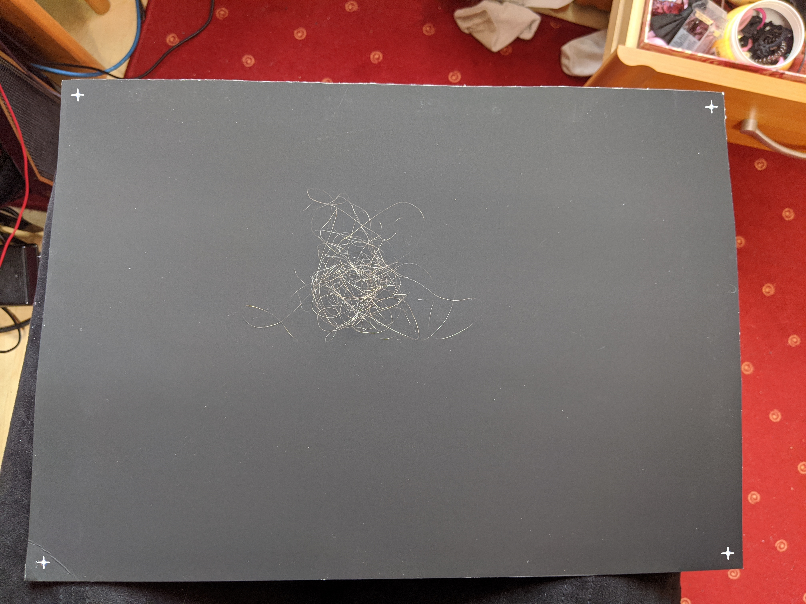
\includegraphics[width=\linewidth]{figBina/01foundDots.png}
		\caption{Input} \label{fig:a}
	\end{subfigure}\hspace*{\fill}
	\begin{subfigure}{0.48\textwidth}
		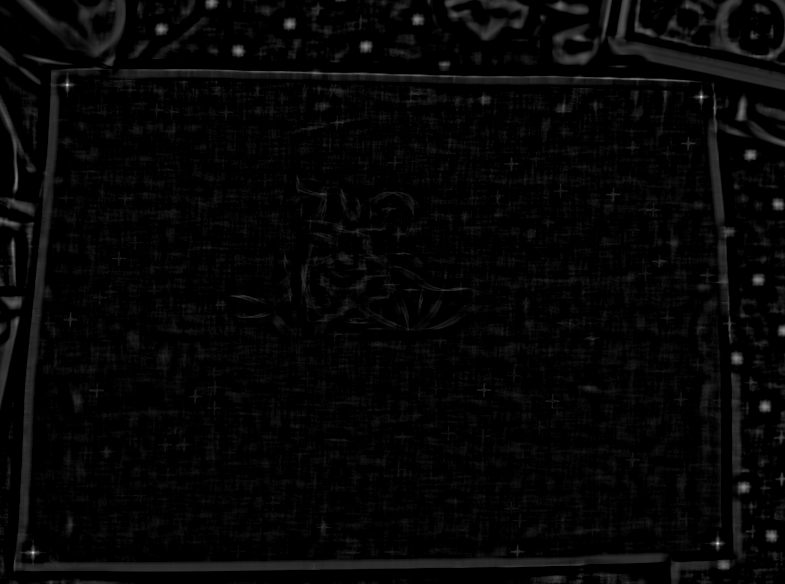
\includegraphics[width=\linewidth]{figBina/02revRes.png}
		\caption{Wahrscheinlichkeiten von matchTemplate} \label{fig:b}
	\end{subfigure}
	
	\medskip
	\begin{subfigure}{0.48\textwidth}
		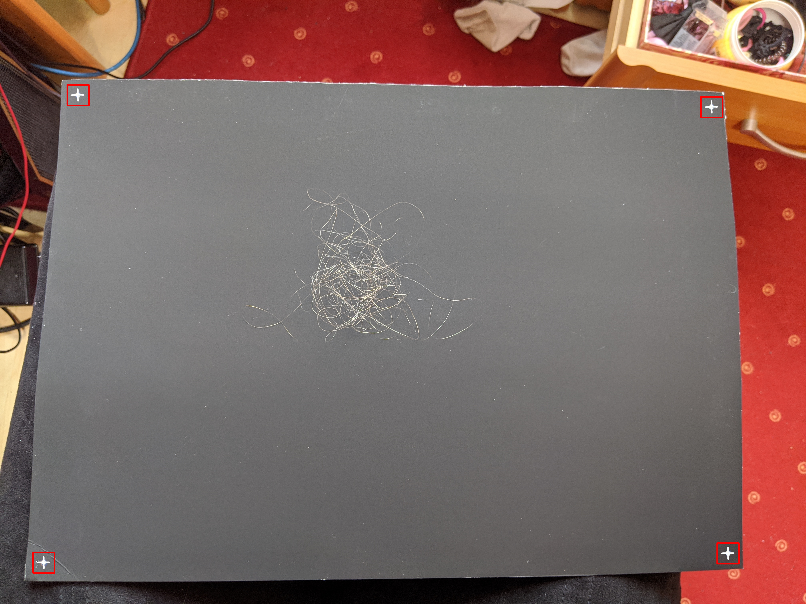
\includegraphics[width=\linewidth]{figBina/02foundDots.png}
		\caption{4 gefundene Markierungen} \label{fig:c}
	\end{subfigure}\hspace*{\fill}
	\begin{subfigure}{0.48\textwidth}
		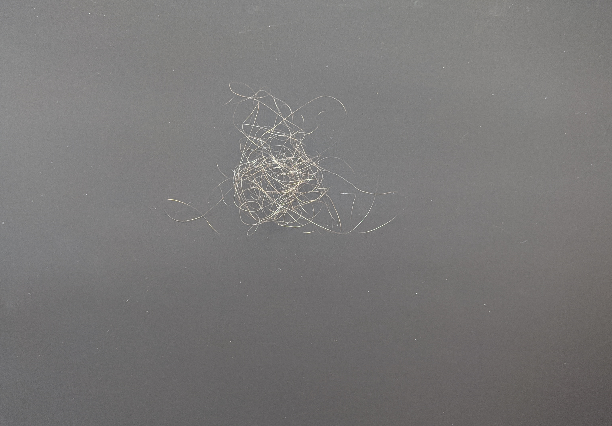
\includegraphics[width=\linewidth]{figBina/03crop image.png}
		\caption{Auf Markierungen zugeschnitten} \label{fig:d}
	\end{subfigure}
	
	\medskip
	\begin{subfigure}{0.48\textwidth}
		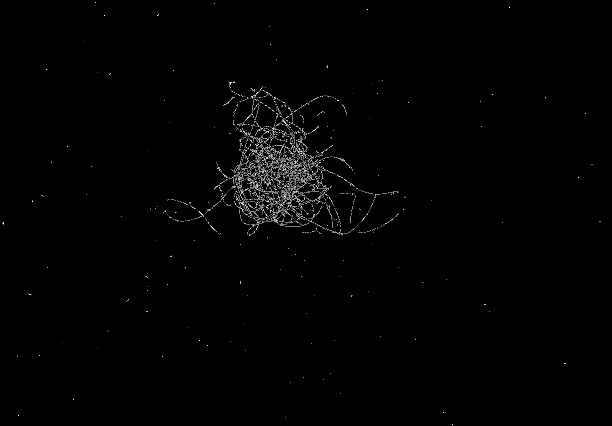
\includegraphics[width=\linewidth]{figBina/04edges.png}
		\caption{Kantendetektion} \label{fig:e}
	\end{subfigure}\hspace*{\fill}
	\begin{subfigure}{0.48\textwidth}
		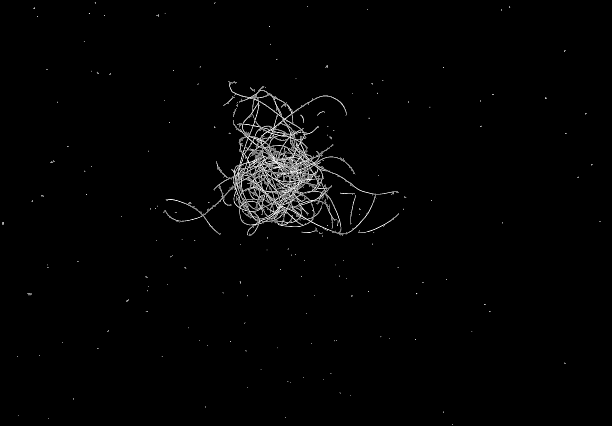
\includegraphics[width=\linewidth]{figBina/05intenstiy.png}
		\caption{Intensität} \label{fig:BinaRawIntensity}
	\end{subfigure}
	
	
	\caption{My complicated figure} \label{fig:1}
\end{figure}

\begin{figure}[H] % "[t!]" placement specifier just for this example
	\begin{subfigure}{0.48\textwidth}
		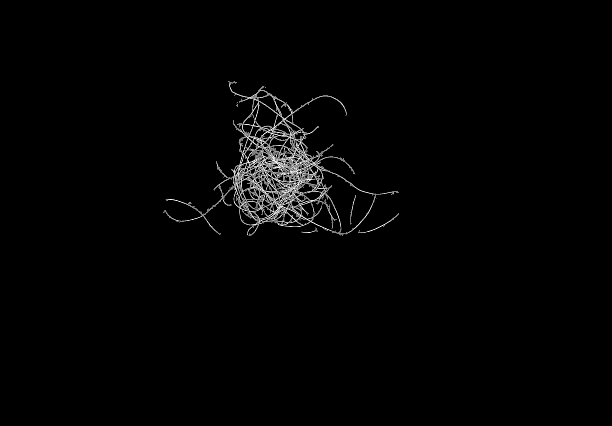
\includegraphics[width=\linewidth]{figBina/06small regions removed.png}
		\caption{Kleine Regionen entfernt} \label{fig:a}
	\end{subfigure}\hspace*{\fill}
	\begin{subfigure}{0.48\textwidth}
		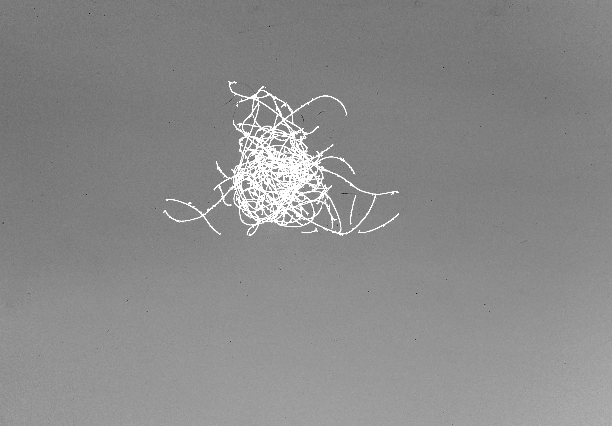
\includegraphics[width=\linewidth]{figBina/07missed hair.png}
		\caption{Intensität auf Input(Grayscale) ausgegeben. Zeigt wie viele Haare nicht erkannt wurden (hier: nicht viele)} \label{fig:b}
	\end{subfigure}
	
	\medskip
	\begin{subfigure}{0.48\textwidth}
		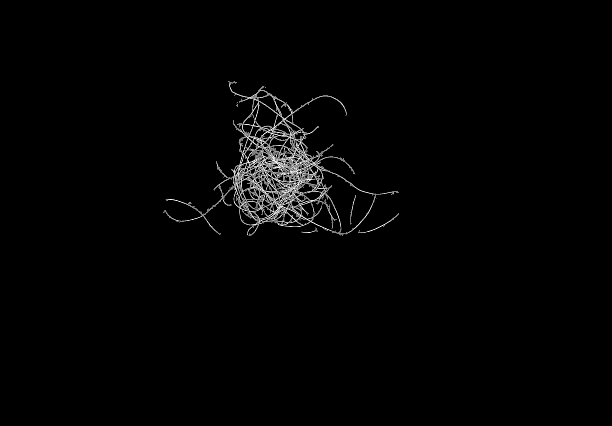
\includegraphics[width=\linewidth]{figBina/08input intensity.png}
		\caption{Intensität-Bild dient als Input für Hintergrund-Region-Untersuchung} \label{fig:c}
	\end{subfigure}\hspace*{\fill}
	\begin{subfigure}{0.48\textwidth}
		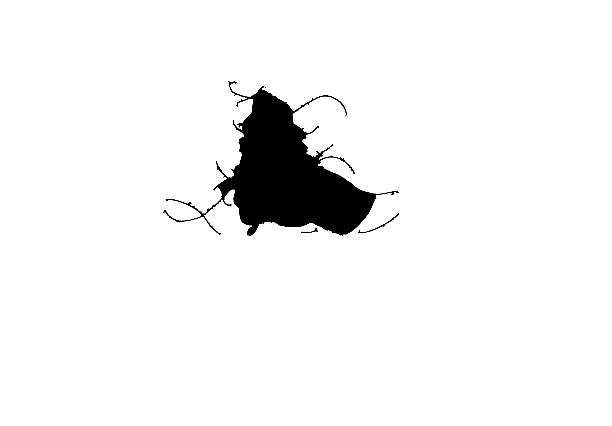
\includegraphics[width=\linewidth]{figBina/08outer section.png}
		\caption{Hintergrund Region, die die Haare umschließt, in weiß} \label{fig:d}
	\end{subfigure}
	
	\medskip
	\begin{subfigure}{0.48\textwidth}
		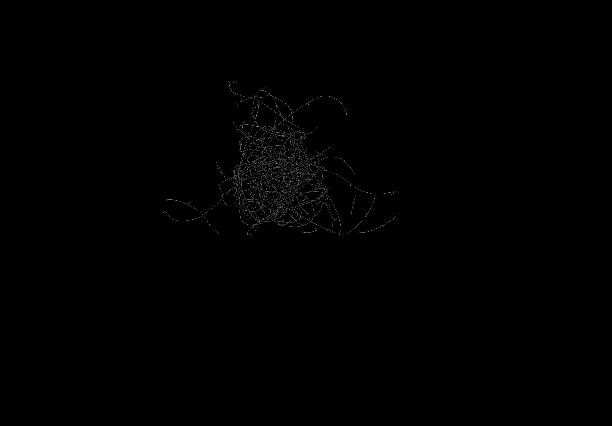
\includegraphics[width=\linewidth]{figBina/09input intensity.png}
		\caption{Intensität-Bild nach Skelettierung. Input für 2. Hintergrund Untersuchung} \label{fig:e}
	\end{subfigure}\hspace*{\fill}
	\begin{subfigure}{0.48\textwidth}
		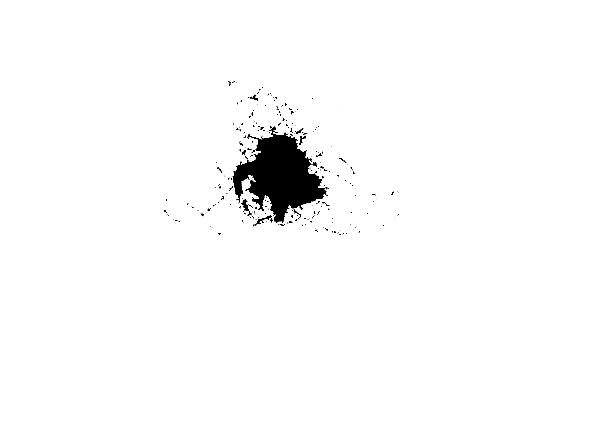
\includegraphics[width=\linewidth]{figBina/09outer section.png}
		\caption{Hintergrund Region, die dichte Haare umschließt} \label{fig:f}
	\end{subfigure}
	
	
	\caption{My complicated figure} \label{fig:1}
\end{figure}


\section{Schätzungs-Modelle Blondes Haar}
\label{appendix:Blond}
\begin{figure}[H] % "[t!]" placement specifier just for this example
	\begin{subfigure}{0.48\textwidth}
		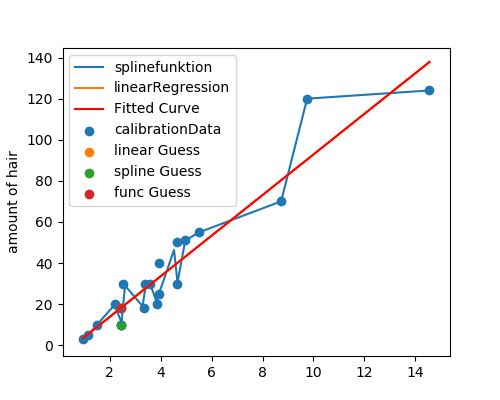
\includegraphics[width=1.1\linewidth]{figBina/g1.png}
		\caption{hairpercent} \label{fig:a}
	\end{subfigure}\hspace*{\fill}
	\begin{subfigure}{0.48\textwidth}
		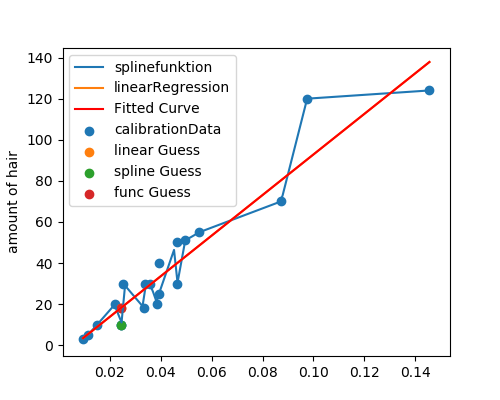
\includegraphics[width=1.1\linewidth]{figBina/g2.png}
		\caption{density*hairsection size} \label{fig:b}
	\end{subfigure}
	
	\medskip
	\begin{subfigure}{0.48\textwidth}
		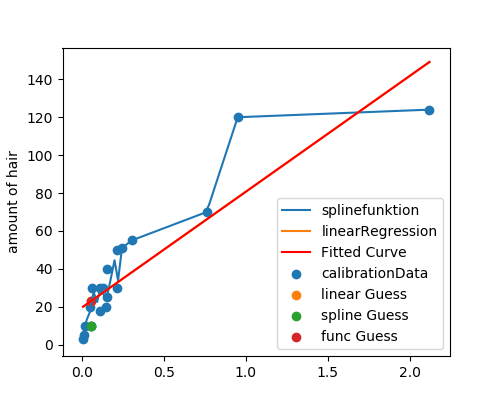
\includegraphics[width=1.1\linewidth]{figBina/g3.png}
		\caption{density per sectionsize per hairperc} \label{fig:c}
	\end{subfigure}\hspace*{\fill}
	\begin{subfigure}{0.48\textwidth}
		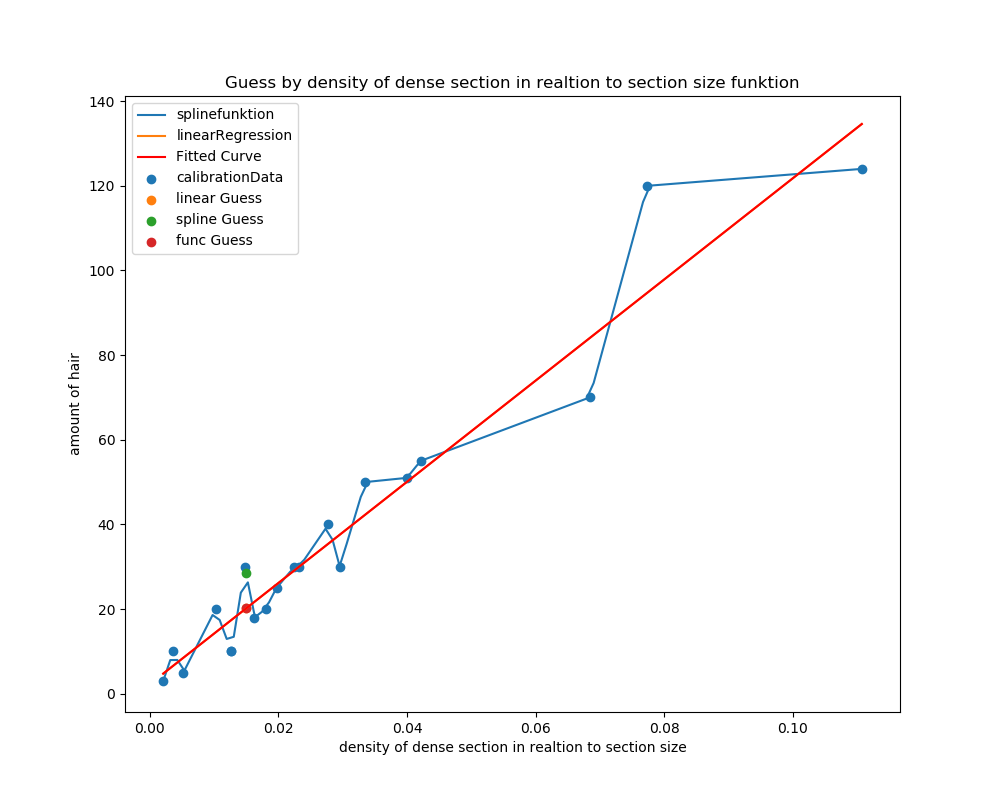
\includegraphics[width=1.1\linewidth]{figBina/g4.png}
		\caption{density of dense section in relation to section size} \label{fig:d}
	\end{subfigure}
	
	\medskip
	\begin{subfigure}{0.48\textwidth}
		\includegraphics[width=1.1\linewidth]{figBina/g5.png}
		\caption{dense Density to loose Density ratio} \label{fig:e}
	\end{subfigure}\hspace*{\fill}
	\begin{subfigure}{0.48\textwidth}
		\includegraphics[width=1.1\linewidth]{figBina/g6.png}
		\caption{density by background section peeking through} \label{fig:f}
	\end{subfigure}
	
	
	\caption{Schätzungsmodelle angewandt auf feine blonde Haare (1)} \label{fig:1}
\end{figure}

\begin{figure}[H] % "[t!]" placement specifier just for this example
	\begin{subfigure}{0.48\textwidth}
		\includegraphics[width=1.1\linewidth]{figBina/g7.png}
		\caption{hairpercent} \label{fig:a}
	\end{subfigure}\hspace*{\fill}
	\begin{subfigure}{0.48\textwidth}
		\includegraphics[width=1.1\linewidth]{figBina/g8.png}
		\caption{density*hairsection size} \label{fig:b}
	\end{subfigure}
	
	\medskip
	\begin{subfigure}{0.48\textwidth}
		\includegraphics[width=1.1\linewidth]{figBina/g9.png}
		\caption{density per sectionsize per hairperc} \label{fig:c}
	\end{subfigure}\hspace*{\fill}
	\begin{subfigure}{0.48\textwidth}
		\includegraphics[width=1.1\linewidth]{figBina/g10.png}
		\caption{density of dense section in relation to section size} \label{fig:d}
	\end{subfigure}
	
	\medskip
	\begin{subfigure}{0.48\textwidth}
		\includegraphics[width=1.1\linewidth]{figBina/g11.png}
		\caption{dense Density to loose Density ratio} \label{fig:e}
	\end{subfigure}\hspace*{\fill}
	\begin{subfigure}{0.48\textwidth}
		\includegraphics[width=1.1\linewidth]{figBina/g12.png}
		\caption{density by background section peeking through} \label{fig:f}
	\end{subfigure}
	
	
	\caption{Schätzungsmodelle angewandt auf feine blonde Haare (2)} \label{fig:1}
\end{figure}

\section{Fehler bei den Schätzungen}
\label{appendix:Error}

lange Rotbraune Haare:

\begin{itemize}
	\item calibration images ['15' '15' '18' '22' '22' '25' '30' '30' '37' '40' '60' '95']
	\item estimated [27 22 23 22 67 17 23 16 28 19 17 14 13 20 27 26 89 25 13 23 19 14 13 34 
	21 16 56 27 20] estimated
	\item (estimated, actual)
	[(27, 22), (22, 22), (23, 25), (22, 18), (67, 65), (17, 22), (23, 22), (16, 18), (28, 26), (19, 21), (17, 18), (14, 9), (13, 17), (20, 27), (27, 30), (26, 27), (89, 95), (25, 40), (13, 15), (23, 31), (19, 31), (14, 11), (13, 16), (34, 50), (21, 30), (16, 12), (56, 45), (27, 34), (20, 16)]
	\item error per estimation [  5   0  -2   4   2  -5   1  -2   2  -2  -1   5  -4  -7  -3  -1  -6 -15
	-2  -8 -12   3  -3 -16  -9   4  11  -7   4]
	\item mean error 5.0344827586206895
\end{itemize}

lange Rotbraune Haare mit kleinerem Kalibrations-Raum:

\begin{itemize}
	\item calibration images ['15' '60' '95']
	\item estimated [30 26 25 23 81 14 22  9 33 17 12  9  8 19 24 28 94 26  7 23 16  6  6 39
	18 10 62 31 19] 
	\item (estimated, actual)
	[(30, 22), (26, 22), (25, 25), (23, 18), (81, 65), (14, 22), (22, 22), (9, 18), (33, 26), (17, 21), (12, 18), (9, 9), (8, 17), (19, 27), (24, 30), (28, 27), (94, 95), (26, 40), (7, 15), (23, 31), (16, 31), (6, 11), (6, 16), (39, 50), (18, 30), (10, 12), (62, 45), (31, 34), (19, 16)]
	\item error per estimation [  8   4   0   5  16  -8   0  -9   7  -4  -6   0  -9  -8  -6   1  -1 -14
	-8  -8 -15  -5 -10 -11 -12  -2  17  -3   3]
	\item mean error 6.896551724137931
\end{itemize}

Blonde lange,feine Haare:
\begin{itemize}
	\item calibration images ['124' '18' '40' '5']
	\item estimated [ 18   9  18  82 125  19  14  24  24   5  27  19  26  37  34   6  37  44
	44  73]
	\item (estimated, actual)
	[(18, 10), (9, 10), (18, 10), (82, 120), (125, 124), (19, 18), (14, 20), (24, 20), (24, 25), (5, 3), (27, 30), (19, 30), (26, 30), (37, 30), (34, 40), (6, 3), (37, 50), (44, 51), (44, 55), (73, 70)]
	\item error per estimation [  8  -1   8 -38   1   1  -6   4  -1   2  -3 -11  -4   7  -6   3 -13  -7
	-11   3]
	\item mean error 6.9
\end{itemize}


Kurze Hellbraune Haare: 

\begin{itemize}
	\item calibration images ['10' '20' '40']
	\item estimated [ 8 10 14 20 16 31 36 40 37 10]
	\item (estimated, actual)
	[(8, 5), (10, 10), (14, 14), (20, 20), (16, 20), (31, 30), (36, 30), (40, 40), (37, 40), (10, 7)]
	\item error per estimation [ 3  0  0  0 -4  1  6  0 -3  3]
	\item mean error 2.0
\end{itemize}

Kurz Dunkelbraune Haare:
\begin{itemize}
	\item calibration images ['15' '22' '25' '6']
	\item estimated [22  8 13 22 17 10 16 16 21 23  6]
	\item (estimated, actual) [(22, 22), (8, 5), (13, 10), (22, 22), (17, 22), (10, 10), (16, 15), (16, 20), (21, 22), (23, 25), (6, 6)]
	\item error per estimation [ 0  3  3  0 -5  0  1 -4 -1 -2  0]
	\item mean error 1.7272727272727273
\end{itemize}


\section{Bedienung}
\label{appendix:bedienung}

Estimation.py ist python script das über die Kommandozeile angesteuert werden kann.

Kalibrierungsdaten und die Ergebnisse von schätzungen werden für einen Nutzer in dem Order Users/NutzerName/data gespeichert.
Um Nutzer anzulegen und zu verwalten gibt es die Kommandos create, switch, user und allUsers. 

\begin{lstlisting}[style=DOS]
D:\Eigene Dateien\Dokumente\GitHub\HairEstimation
\HairEstimationPython>python Estimation.py create UserName
active user: Mummel

adding user UserName
switching to user UserName
\end{lstlisting}

In den Ordner Users/NutzerName/calibrationImages können nachdem ein Nutzer erstellt wurde Bilder für die Kalibierung eingegeben werden. Dabei muss die Anzahl der Haare auf dem Bild gezählt werden und als erste Zahl im Namen der Datei stehen.

\begin{figure}
	\centering
	\includegraphics[width=1.0\textwidth]{figBedienung/calibrationImages.PNG}
	\caption[]{NutzerName/calibrationImages input der Bilder}
\end{figure} 

In Users/UserName muss eine Bilddatei hingelegt werden, die als Template für die Markierungen in den Ecken der Bilder dient.

Mit dem Kommando calibrate wird die Kalibrierung durchgeführt. Mit dem Argument --time kann die Zeit angegeben werden, die jeweils für die Bildverarbeitung gebraucht wird angezeigt. Mit --debug werden die Zwischenschritte der Bildverarbeitung angezeigt.
Mit calibrationResult können die Schätzungs-Modelle, die aus der Kalibrierung resultieren angezeigt werden.
In der Text Datei Users/NutzerName/data/guessfunctions.txt kann für jeden der Modelle ein Funktionstyp für die Fitted Curve angegeben werden.

Nach der Kalibrierung kann ein Bild geschätzt werden.
Einzelne Bilder können über den commando guess Geschätzt werden.
Dabei folgt der Aufruf folgendes muster:

guess relativerPfad-zum-Bild (days) (tag)
 
Das Datum muss als Erste Zahlenkette in dem Dateinamen zu finden sein.

\begin{lstlisting}[style=DOS]
 guess Users/UserName/MyEstimationImages/
 IMG_20200316_132015_18.jpg 2 hairwash
\end{lstlisting}

Dabei müssen days und tag nicht angegeben werden. Days gibt an, über wie viele Tage die Haare gesammelt wurden und tag für eine Markierung für den/die Tage an, die zu der Schätzung gehören.
Mit guessFolder (Pfad) werden alle Bilder geschätzt, die sich in einem Ordner befinden.
Bei guess und guessFolder können wie bei calibrate die Argument --time und --debug genutzt werden.
Zusätzlich kann mit --replace, --mean, --ignore, --keep und --add angegeben werden, wie mit Schätzungen umgegagen werden soll, die zu einem Datum gehören, für den es schon ein Schätzung gibt.

Mit dem Kommando plot wird der zeitliche Verlauf Schätzungen als Graph angezeigt. Mit printResult wird dasselbe in Text Form ausgegeben.

Die letzte Schätzung kann mit removeLastGuess entfernt werden. Mit clearSave werden alle Schätzungen gelöscht.

Die Kommandos calculateError, fullTest und onlyGuessTest wurden genutzt um Fehlerraten zu bestimmen. 

\end{document}